% Options for packages loaded elsewhere
\PassOptionsToPackage{unicode}{hyperref}
\PassOptionsToPackage{hyphens}{url}
%
\documentclass[
  english,
]{book}
\usepackage{amsmath,amssymb}
\usepackage{lmodern}
\usepackage{ifxetex,ifluatex}
\ifnum 0\ifxetex 1\fi\ifluatex 1\fi=0 % if pdftex
  \usepackage[T1]{fontenc}
  \usepackage[utf8]{inputenc}
  \usepackage{textcomp} % provide euro and other symbols
\else % if luatex or xetex
  \usepackage{unicode-math}
  \defaultfontfeatures{Scale=MatchLowercase}
  \defaultfontfeatures[\rmfamily]{Ligatures=TeX,Scale=1}
\fi
% Use upquote if available, for straight quotes in verbatim environments
\IfFileExists{upquote.sty}{\usepackage{upquote}}{}
\IfFileExists{microtype.sty}{% use microtype if available
  \usepackage[]{microtype}
  \UseMicrotypeSet[protrusion]{basicmath} % disable protrusion for tt fonts
}{}
\makeatletter
\@ifundefined{KOMAClassName}{% if non-KOMA class
  \IfFileExists{parskip.sty}{%
    \usepackage{parskip}
  }{% else
    \setlength{\parindent}{0pt}
    \setlength{\parskip}{6pt plus 2pt minus 1pt}}
}{% if KOMA class
  \KOMAoptions{parskip=half}}
\makeatother
\usepackage{xcolor}
\IfFileExists{xurl.sty}{\usepackage{xurl}}{} % add URL line breaks if available
\IfFileExists{bookmark.sty}{\usepackage{bookmark}}{\usepackage{hyperref}}
\hypersetup{
  pdftitle={DRAFT: ReCentering Psych Stats: Multivariate Modeling},
  pdfauthor={Lynette H Bikos, PhD, ABPP},
  pdflang={en},
  hidelinks,
  pdfcreator={LaTeX via pandoc}}
\urlstyle{same} % disable monospaced font for URLs
\usepackage{color}
\usepackage{fancyvrb}
\newcommand{\VerbBar}{|}
\newcommand{\VERB}{\Verb[commandchars=\\\{\}]}
\DefineVerbatimEnvironment{Highlighting}{Verbatim}{commandchars=\\\{\}}
% Add ',fontsize=\small' for more characters per line
\usepackage{framed}
\definecolor{shadecolor}{RGB}{248,248,248}
\newenvironment{Shaded}{\begin{snugshade}}{\end{snugshade}}
\newcommand{\AlertTok}[1]{\textcolor[rgb]{0.94,0.16,0.16}{#1}}
\newcommand{\AnnotationTok}[1]{\textcolor[rgb]{0.56,0.35,0.01}{\textbf{\textit{#1}}}}
\newcommand{\AttributeTok}[1]{\textcolor[rgb]{0.77,0.63,0.00}{#1}}
\newcommand{\BaseNTok}[1]{\textcolor[rgb]{0.00,0.00,0.81}{#1}}
\newcommand{\BuiltInTok}[1]{#1}
\newcommand{\CharTok}[1]{\textcolor[rgb]{0.31,0.60,0.02}{#1}}
\newcommand{\CommentTok}[1]{\textcolor[rgb]{0.56,0.35,0.01}{\textit{#1}}}
\newcommand{\CommentVarTok}[1]{\textcolor[rgb]{0.56,0.35,0.01}{\textbf{\textit{#1}}}}
\newcommand{\ConstantTok}[1]{\textcolor[rgb]{0.00,0.00,0.00}{#1}}
\newcommand{\ControlFlowTok}[1]{\textcolor[rgb]{0.13,0.29,0.53}{\textbf{#1}}}
\newcommand{\DataTypeTok}[1]{\textcolor[rgb]{0.13,0.29,0.53}{#1}}
\newcommand{\DecValTok}[1]{\textcolor[rgb]{0.00,0.00,0.81}{#1}}
\newcommand{\DocumentationTok}[1]{\textcolor[rgb]{0.56,0.35,0.01}{\textbf{\textit{#1}}}}
\newcommand{\ErrorTok}[1]{\textcolor[rgb]{0.64,0.00,0.00}{\textbf{#1}}}
\newcommand{\ExtensionTok}[1]{#1}
\newcommand{\FloatTok}[1]{\textcolor[rgb]{0.00,0.00,0.81}{#1}}
\newcommand{\FunctionTok}[1]{\textcolor[rgb]{0.00,0.00,0.00}{#1}}
\newcommand{\ImportTok}[1]{#1}
\newcommand{\InformationTok}[1]{\textcolor[rgb]{0.56,0.35,0.01}{\textbf{\textit{#1}}}}
\newcommand{\KeywordTok}[1]{\textcolor[rgb]{0.13,0.29,0.53}{\textbf{#1}}}
\newcommand{\NormalTok}[1]{#1}
\newcommand{\OperatorTok}[1]{\textcolor[rgb]{0.81,0.36,0.00}{\textbf{#1}}}
\newcommand{\OtherTok}[1]{\textcolor[rgb]{0.56,0.35,0.01}{#1}}
\newcommand{\PreprocessorTok}[1]{\textcolor[rgb]{0.56,0.35,0.01}{\textit{#1}}}
\newcommand{\RegionMarkerTok}[1]{#1}
\newcommand{\SpecialCharTok}[1]{\textcolor[rgb]{0.00,0.00,0.00}{#1}}
\newcommand{\SpecialStringTok}[1]{\textcolor[rgb]{0.31,0.60,0.02}{#1}}
\newcommand{\StringTok}[1]{\textcolor[rgb]{0.31,0.60,0.02}{#1}}
\newcommand{\VariableTok}[1]{\textcolor[rgb]{0.00,0.00,0.00}{#1}}
\newcommand{\VerbatimStringTok}[1]{\textcolor[rgb]{0.31,0.60,0.02}{#1}}
\newcommand{\WarningTok}[1]{\textcolor[rgb]{0.56,0.35,0.01}{\textbf{\textit{#1}}}}
\usepackage{longtable,booktabs,array}
\usepackage{calc} % for calculating minipage widths
% Correct order of tables after \paragraph or \subparagraph
\usepackage{etoolbox}
\makeatletter
\patchcmd\longtable{\par}{\if@noskipsec\mbox{}\fi\par}{}{}
\makeatother
% Allow footnotes in longtable head/foot
\IfFileExists{footnotehyper.sty}{\usepackage{footnotehyper}}{\usepackage{footnote}}
\makesavenoteenv{longtable}
\usepackage{graphicx}
\makeatletter
\def\maxwidth{\ifdim\Gin@nat@width>\linewidth\linewidth\else\Gin@nat@width\fi}
\def\maxheight{\ifdim\Gin@nat@height>\textheight\textheight\else\Gin@nat@height\fi}
\makeatother
% Scale images if necessary, so that they will not overflow the page
% margins by default, and it is still possible to overwrite the defaults
% using explicit options in \includegraphics[width, height, ...]{}
\setkeys{Gin}{width=\maxwidth,height=\maxheight,keepaspectratio}
% Set default figure placement to htbp
\makeatletter
\def\fps@figure{htbp}
\makeatother
\setlength{\emergencystretch}{3em} % prevent overfull lines
\providecommand{\tightlist}{%
  \setlength{\itemsep}{0pt}\setlength{\parskip}{0pt}}
\setcounter{secnumdepth}{5}
\usepackage{booktabs}
\ifxetex
  % Load polyglossia as late as possible: uses bidi with RTL langages (e.g. Hebrew, Arabic)
  \usepackage{polyglossia}
  \setmainlanguage[]{english}
\else
  \usepackage[main=english]{babel}
% get rid of language-specific shorthands (see #6817):
\let\LanguageShortHands\languageshorthands
\def\languageshorthands#1{}
\fi
\ifluatex
  \usepackage{selnolig}  % disable illegal ligatures
\fi
\usepackage[]{natbib}
\bibliographystyle{plainnat}

\title{DRAFT: ReCentering Psych Stats: Multivariate Modeling}
\author{Lynette H Bikos, PhD, ABPP}
\date{}

\begin{document}
\maketitle

{
\setcounter{tocdepth}{1}
\tableofcontents
}
\hypertarget{book-cover}{%
\chapter*{BOOK COVER}\label{book-cover}}
\addcontentsline{toc}{chapter}{BOOK COVER}

\begin{figure}
\centering
\includegraphics{images/ReC_multivariate_bkcvr.png}
\caption{An image of the book cover. It includes four quadrants of non-normal distributions representing gender, race/ethnicty, sustainability/global concerns, and journal articles}
\end{figure}

\hypertarget{preface}{%
\chapter*{PREFACE}\label{preface}}
\addcontentsline{toc}{chapter}{PREFACE}

\textbf{If you are viewing this document, you should know that this is a book-in-progress. Early drafts are released for the purpose teaching my classes and gaining formative feedback from a host of stakeholders. The document was last updated on 23 Mar 2021}

To \emph{center} a variable in regression means to set its value at zero and interpret all other values in relation to this reference point. Regarding race and gender, researchers often center male and White at zero. Further, it is typical that research vignettes in statistics textbooks are similarly seated in a White, Western (frequently U.S.), heteronormative, framework. The purpose of this project is to create a set of open educational resources (OER) appropriate for doctoral and post-doctoral training that contribute to justice, equity, diversity, inclusion (JEDI), and social responsivity.

Statistics training in doctoral programs are frequently taught with fee-for-use programs (e.g., SPSS/AMOS, SAS, MPlus) that may not be readily available to the post-doctoral professional. In recent years, there has been an increase and improvement in R packages (e.g., \emph{psych}, \emph{lavaan}) used for in analyses common to psychological research. Correspondingly, many graduate programs are transitioning to statistics training in R (free and open source). This is a challenge for post-doctoral psychologists who were trained with other software. This OER will offer statistics training with R and be, freely available on open science platforms under a Creative Commons Attribution - Non Commercial - Share Alike license {[}CC BY-NC-SA 4.0{]}.

Training models for doctoral programs in HSP are commonly scholar-practitioner, scientist-practitioner, or clinical-scientist. An emerging model, the \emph{scientist-practitioner-advocacy} training model incorporates social justice advocacy so that graduates are equipped to recognize and address the sociocultural context of oppression and unjust distribution of resources and opportunities \citep{mallinckrodt_scientist-practitioner-advocate_2014}. In statistics textbooks, the use of research vignettes engages the learner around a tangible scenario for identifying independent variables, dependent variables, covariates, and potential mechanisms of change. Many students recall examples in Field's \citeyearpar{field_discovering_2012} popular statistics text: Viagra to teach one-way ANOVA, beer goggles for two-way ANOVA, and bushtucker for repeated measures. What if the research vignettes were investigations around JEDI/social responsivity and highlighted the scholarship of individuals whose identities are often marginalized?

In this OER, research vignettes will be from recently published articles where: (a) the author's identity is from a group where scholarship is historically marginalized (e.g., BIPOC, LGBTQ+, emerging nations), (b) the research has a JEDI/social responsivity focus, (b) the lesson's statistic is used in the article, and (c) the data is shared publicly or there is sufficient information in the article to simulate the data for the chapter example(s) and practice problem(s).

\hypertarget{copyright-with-open-access}{%
\section*{Copyright with Open Access}\label{copyright-with-open-access}}
\addcontentsline{toc}{section}{Copyright with Open Access}

This book is published under a a Creative Commons Attribution-NonCommercial-ShareAlike 4.0 International License. This means that this book can be reused, remixed, retained, revised and redistributed (including commercially) as long as appropriate credit is given to the authors. If you remix, or modify the original version of this open textbook, you must redistribute all versions of this open textbook under the same license - CC BY-SA.

Our GitHub open-source repository contains all of the text and source code for the book, including data and images.

\hypertarget{ReCintro}{%
\chapter{Introduction}\label{ReCintro}}

\hypertarget{what-to-expect-in-each-chapter}{%
\section{What to expect in each chapter}\label{what-to-expect-in-each-chapter}}

This textbook is intended as \emph{applied,} in that a primary goal is to help the scientist-practitioner-advocate use the statistic in a research problem and \emph{write it up} for a program evaluation, dissertation, or journal article. In support of that goal, I try to provide \emph{just enough} conceptual information so that the researcher can select the appropriate statistic (i.e., distinguishing between when ANOVA is appropriate and when regression is appropriate) and assign variables to their proper role (e.g., covariate, moderator, mediator).

This conceptual approach does include step-by-step \emph{hand-calculations} (only we calculate them arithmetically in R) to provide a \emph{visceral feeling} of what is happening within the statistical algorithm that may be invisible to the researcher. Additionally, the conceptual review includes a review of the assumptions about the characteristics of the data and research design that are required for the statistic. Statistics can be daunting, so I have worked hard to establish a \emph{workflow} through each analysis. When possible, I include a flowchart that is referenced frequently in each chapter and assists the the researcher keep track of their place in the many steps and choices that accompany even the simplest of analyses.

As with many statistics texts, each chapter includes a \emph{research vignette.} Somewhat unique to this resource is that the vignettes are selected from recently published articles. Each vignette is chosen with the intent to meet as many of the following criteria as possible:

\begin{itemize}
\tightlist
\item
  the statistic that is the focus of the chapter was properly used in the article,
\item
  the author's identity is from a group where scholarship is historically marginalized (e.g., BIPOC, LGBTQ+, emerging nations),
\item
  the research has a justice, equity, inclusion, diversity, and social responsivity focus and will contribute positively to a social justice pedagogy, and
\item
  the data is available in a repository or there is sufficient information in the article to simulate the data for the chapter example(s) and practice problem(s).
\end{itemize}

In each chapter we employ \emph{R} packages that will efficiently calculate the statistic and the dashboard of metrics (e.g., effect sizes, confidence intervals) that are typically reported in psychological science.

\hypertarget{if-you-are-new-to-r}{%
\section{If You are New to R}\label{if-you-are-new-to-r}}

In this section I will provide some orientation to using R in psychological research. I don't intend this text to be ``R from the ground up,'' but I will provide enough guidance that the individual can start working the problems.

I will also link to tutorials that help individuals get started in R.

\hypertarget{r-hygiene}{%
\subsection{R Hygiene}\label{r-hygiene}}

Many problems in R can be resolved with good ``R hygiene.'' I will review those practices here. I will also review the conventions I will try to consistently use throughout the text.

Everything in a folder

Although it is often considered good R etiquette to load all packages at the beginning of the script, this is not my practice. Each chapter will include a script that lists all the packages used, but I will open each package as we use it. This will provide a greater sense of which packages are needed for what task.

\hypertarget{maximizing-learning-by-accessing-all-the-resources}{%
\section{Maximizing Learning by Accessing all the Resources}\label{maximizing-learning-by-accessing-all-the-resources}}

In this section I will talk about the options for using and learning the materials. Primarily these are:

\begin{enumerate}
\def\labelenumi{\arabic{enumi}.}
\tightlist
\item
  Open a new document of R, copying the script over and running it in a fresh document.
\item
  Forking the entire suite of materials from GitHub and working directly in the original R markdown documents with the option to annotate the material directly.
\item
  Forking the materials to adopt and or adapt for teaching.
\item
  Listening to the accompanying lectures (I sound best when the speed is 1.75). I intend to record the lectures in Panopto which provides some closed captioning options.
\item
  Making use of the practice problems.
\end{enumerate}

\hypertarget{dataprep}{%
\chapter*{DATA PREP}\label{dataprep}}
\addcontentsline{toc}{chapter}{DATA PREP}

\hypertarget{scrub}{%
\chapter{Scrubbing}\label{scrub}}

{[}Screencasted Lecture Link{]}

The focus of this chapter is the process of starting with raw data and preparing it for multivariate analysis. To that end, we will address the conceptual considerations and practical steps in ``scrubbing and scoring.''

A twist in this lesson is that we are asking you to contribute to the dataset that serves as the basis for the chapter and the practice problems. In the spirit of \emph{open science}, this dataset is available to you and others for your own learning. Before continuing, please take 15-20 minutes to complete the survey titled, \href{https://spupsych.az1.qualtrics.com/jfe/form/SV_b2cClqAlLGQ6nLU}{Rate-a-Recent-Course: A ReCentering Psych Stats Exercise}. The study is approved by the Institutional Review Board at Seattle Pacific University (SPUIRB\# 202102011, no expiration). Details about the study, including an informed consent, are included at the link.

\hypertarget{navigating-this-lesson}{%
\section{Navigating this Lesson}\label{navigating-this-lesson}}

There is about \# hours and \#\# minutes of lecture. If you work through the materials with me it would be good to add another \#\# hours.

\hypertarget{learning-objectives}{%
\subsection{Learning Objectives}\label{learning-objectives}}

Learning objectives from this lecture include the following:

\begin{itemize}
\tightlist
\item
  Import data from Qualtrics into R.
\item
  Begin the scrubbing process by applying exclusion and inclusion criteria.
\item
  Rename variables.
\item
  Create a smaller dataframe with variables appropriate for testing a specific statistical model.
\item
  Use critical data manipulation functions from the \emph{tidyverse} (and \emph{dplyr}) in particular such as \emph{filter()}, \emph{select()}, and \emph{mutate()} to prepare variables.
\item
  Articulate the initial steps in a workflow for scrubbing and scoring data.
\end{itemize}

\hypertarget{planning-for-practice}{%
\subsection{Planning for Practice}\label{planning-for-practice}}

The suggestions for practice will start with this chapter and continue in the next two chapters (Scoring, Data Dx). Using Parent's \citeyearpar{parent_handling_2013} AIA approach to managing missing data, you will scrub-and-score a raw dataset. Options of graded complexity could incude:

\begin{itemize}
\tightlist
\item
  Repeating the steps in the chapter with the most recent data from the Rate-A-Recent-Course survey; differences will be in the number of people who have completed the survey since the chapter was written.
\item
  Use the dataset that is the source of the chapter, but score a different set of items that you choose.
\item
  Begin with raw data to which you have access.
\end{itemize}

\hypertarget{readings-resources}{%
\subsection{Readings \& Resources}\label{readings-resources}}

In preparing this chapter, I drew heavily from the following resource(s). Other resources are cited (when possible, linked) in the text with complete citations in the reference list.

\begin{itemize}
\item
  Parent, M. C. (2013). Handling item-level missing data: Simpler is just as good. The Counseling Psychologist, 41(4), 568--600. \url{https://doi.org/10.1177/0011000012445176}
\item
  Kline, R. B. (2015). Data preparation and psychometrics review. In Principles and Practice of Structural Equation Modeling, Fourth Edition. Guilford Publications. \url{http://ebookcentral.proquest.com/lib/spu/detail.action?docID=4000663}
\item
  Grolemund, G., \& Wickham, H. (n.d.). 5 Data transformation \textbar{} R for Data Science. Retrieved March 12, 2020, from \url{https://r4ds.had.co.nz/}
\end{itemize}

\hypertarget{packages}{%
\subsection{Packages}\label{packages}}

The script below will (a) check to see if the following packages are installed on your computer and, if not (b) install them.

\begin{Shaded}
\begin{Highlighting}[]
\CommentTok{\#will install the package if not already installed}
\ControlFlowTok{if}\NormalTok{(}\SpecialCharTok{!}\FunctionTok{require}\NormalTok{(qualtRics))\{}\FunctionTok{install.packages}\NormalTok{(}\StringTok{"qualtRics"}\NormalTok{)\}}
\ControlFlowTok{if}\NormalTok{(}\SpecialCharTok{!}\FunctionTok{require}\NormalTok{(tidyverse))\{}\FunctionTok{install.packages}\NormalTok{(}\StringTok{"tidyverse"}\NormalTok{)\}}
\ControlFlowTok{if}\NormalTok{(}\SpecialCharTok{!}\FunctionTok{require}\NormalTok{(psych))\{}\FunctionTok{install.packages}\NormalTok{(}\StringTok{"psych"}\NormalTok{)\}}
\end{Highlighting}
\end{Shaded}

\hypertarget{workflow-for-scrubbing-and-scoring}{%
\section{Workflow for Scrubbing and Scoring}\label{workflow-for-scrubbing-and-scoring}}

The following is a proposed workflow for preparing data for analysis.

\begin{figure}
\centering
\includegraphics{images/Ch02/scrubscore_wrkflow.jpg}
\caption{An image of a workflow for scrubbing and scoring data.}
\end{figure}

Here is a narration of the figure:

\begin{enumerate}
\def\labelenumi{\arabic{enumi}.}
\tightlist
\item
  The workflow begins by importing data into R. Most lessons in this series involve simulated data that are created directly in R. Alternatively, data could be:

  \begin{itemize}
  \tightlist
  \item
    imported ``intRavenously'' through programs such as Qualtrics,
  \item
    exported from programs such as Qualtrics to another program (e.g., .xlxs, .csv)
  \item
    imported in other forms (e.g., .csv,.sps, .sav).
  \end{itemize}
\item
  Scrubbing data by

  \begin{itemize}
  \tightlist
  \item
    variable naming,
  \item
    specifying variable characteristics such as factoring,
  \item
    ensuring that included particpiants consented to participation,
  \item
    determining and executing the inclusion and exclusion criteria.
  \end{itemize}
\item
  Conduct preliminary data diagnostics such as

  \begin{itemize}
  \tightlist
  \item
    outlier anlaysis
  \item
    assessing for univariate and multivariate analysis
  \item
    making transformations and/or corrections
  \end{itemize}
\item
  Managing missingness by one of two routes

  \begin{itemize}
  \tightlist
  \item
    Available information analysis \citep{parent_handling_2013} at either the item-level or scale level. The result is a single set of data for analysis. If missingness remains, options include pairwise deletion, listwise deletion, or specifying FIML (when available). Another option is to use multiple imputation.
  \item
    Multiple imputation at either scale level or item-level
  \end{itemize}
\end{enumerate}

\hypertarget{research-vignette}{%
\section{Research Vignette}\label{research-vignette}}

To provide first-hand experience as both the respondent and analyst for the same set of data, you were asked to complete a survey titled, \href{https://spupsych.az1.qualtrics.com/jfe/form/SV_b2cClqAlLGQ6nLU}{Rate-a-Recent-Course: A ReCentering Psych Stats Exercise}. If you haven't yet completed it, please consider doing so, now. In order to reduce the potential threats to validity by providing background information about the survey, I will wait to describe it until later in the chapter.

The survey is administered in Qualtrics. In the chapter I teach two ways to import Qualtrics data into R. We will then use the data to work through the steps identified in the workflow.

\hypertarget{working-the-problem}{%
\section{Working the Problem}\label{working-the-problem}}

\hypertarget{intravenous-qualtrics}{%
\subsection{intRavenous Qualtrics}\label{intravenous-qualtrics}}

I will demonstrate using a Qualtrics account at my institution, Seattle Pacific University. The only surveys in this account are for the \emph{Recentering Psych Stats} chapters and lessons. All surveys are designed to not capture personally identifying information.

Access credentials for the institutional account, individual user's account, and survey are essential for getting the survey items and/or results to export into R. The Qualtrics website provides a tutorial for \href{https://www.qualtrics.com/support/integrations/api-integration/overview/\#GeneratingAnAPIToken}{generating an API token}.

We need two pieces of information: the \textbf{root\_url} and an \textbf{API token}.

\begin{itemize}
\tightlist
\item
  Log into your respective qualtrics.com account.
\item
  Select Account Settings
\item
  Choose ``Qualtrics IDs'' from the user name dropdown
\end{itemize}

We need the \textbf{root\_url}. This is the first part of the web address for the Qualtrics account. For our institution it is: spupsych.az1.qualtrics.com

The API token is in the box labeled, ``API.'' If it is empty, select, ``Generate Token.'' If you do not have this option, locate the \emph{brand administrator} for your Qualtrics account. They will need to set up your account so that you have API privileges.

\emph{BE CAREFUL WITH THE API TOKEN} This is the key to your Qualtrics accounts. If you leave it in an .rmd file that you forward to someone else, this key and the base URL gives access to every survey in your account. If you share it, you could be releasing survey data to others that would violate confidentiality promises in an IRB application.

If you mistakenly give out your API token you can generate a new one within your Qualtrics account and re-protect all its contents.

You do need to change the API key/token if you want to download data from a different Qualtrics account. If your list of surveys generates the wrong set of surveys, restart R, make sure you have the correct API token and try again.

\begin{Shaded}
\begin{Highlighting}[]
\CommentTok{\#only have to run this ONCE to draw from the same Qualtrics account...but will need to get different token if you are changing between accounts }
\FunctionTok{library}\NormalTok{(qualtRics)}
\CommentTok{\#qualtrics\_api\_credentials(api\_key = "mUgPMySYkiWpMFkwHale1QE5HNmh5LRUaA8d9PDg",}
              \CommentTok{\#base\_url = "spupsych.az1.qualtrics.com", overwrite = TRUE, install = TRUE)}
\end{Highlighting}
\end{Shaded}

\emph{all\_surveys()} generates a dataframe containing information about all the surveys stored on your Qualtrics account.

\begin{Shaded}
\begin{Highlighting}[]
\NormalTok{surveys }\OtherTok{\textless{}{-}} \FunctionTok{all\_surveys}\NormalTok{() }
\CommentTok{\#View this as an object (found in the right: Environment).  }
\CommentTok{\#Get survey id \# for the next command}
\CommentTok{\#If this is showing you the WRONG list of surveys, you are pulling from the wrong Qualtrics account (i.e., maybe this one instead of your own). Go back and change your API token (it saves your old one). Changing the API likely requires a restart of R.}
\NormalTok{surveys}
\end{Highlighting}
\end{Shaded}

To retrieve the survey, use the \emph{fetch\_survey()} function.

\begin{Shaded}
\begin{Highlighting}[]
\CommentTok{\#obtained with the survey ID \#}
\CommentTok{\#"surveyID" should be the ID from above}
\CommentTok{\#"verbose" prints messages to the R console}
\CommentTok{\#"label", when TRUE, imports data as text responses; if FALSE prints the data as numerical responses}
\CommentTok{\#"convert", when TRUE, attempts to convert certain question types to teh "proper" data type in R; because I don\textquotesingle{}t like guessing, I want to set up my own factors.}
\CommentTok{\#"force\_request", when TRUE, always downloads the survey from the API instead of from a temporary director (i.e., it always goes to the primary source)}
\CommentTok{\# "import\_id", when TRUE includes the unique Qualtrics{-}assigned ID; since I have provided labels, I want false}
\FunctionTok{library}\NormalTok{(qualtRics)}
\NormalTok{QTRX\_df }\OtherTok{\textless{}{-}} \FunctionTok{fetch\_survey}\NormalTok{(}\AttributeTok{surveyID =} \StringTok{"SV\_b2cClqAlLGQ6nLU"}\NormalTok{,}\AttributeTok{useLocalTime =} \ConstantTok{TRUE}\NormalTok{,}
                         \AttributeTok{verbose =} \ConstantTok{FALSE}\NormalTok{, }\AttributeTok{label=}\ConstantTok{FALSE}\NormalTok{, }\AttributeTok{convert=}\ConstantTok{FALSE}\NormalTok{, }\AttributeTok{force\_request =} \ConstantTok{TRUE}\NormalTok{, }\AttributeTok{import\_id =} \ConstantTok{FALSE}\NormalTok{)}
\end{Highlighting}
\end{Shaded}

\emph{It is possible (and helpful, even) to import Qualtrics data that has been downloaded from Qualtrics as a .csv. I demo this in the Bonus Reel.}

\hypertarget{about-the-rate-a-recent-course-survey}{%
\subsection{\texorpdfstring{About the \emph{Rate-a-Recent-Course} Survey}{About the Rate-a-Recent-Course Survey}}\label{about-the-rate-a-recent-course-survey}}

As a teaching activity for the ReCentering Psych Stats OER, the topic of the survey was selected to be consistent with the overall theme of OER. Specifically, the purpose of this study is to understand the campus climate for students whose identities make them vulnerable to bias and discrimination. These include students who are Black, non-Black students of color, LGBTQ+ students, international students, and students with disabilities.

Although the dataset should provide the opportunity to test a number of statistical models, one working hypothesis that framed the study is that the there will be a greater sense of belonging and less bias and discrimination when there is similar representation (of identities that are often marginalized) in the instructional faculty and student body. Termed, ``structural diversity'' \citep{lewis_black_2019} this is likely an oversimplification. In fact, an increase in diverse representation without attention to interacting factors can increase hostility on campus \citep{hurtado_linking_2007}. Thus, we included the task of rating of a single course relates to the larger campus along the dimensions of belonging and bias/discrimination. For example, if a single class has higher ratings on issues of inclusivity, diversity, and respect, we would expect that sentiment to be echoed in the broader institution.

Our design has notable limitations You will likely notice that we ask about demographic characteristics of the instructional staff and classmates in the course rated, but we do not ask about the demographic characteristics of the respondent. In making this decision, we likely lose important information; Iacovino and James \citeyearpar{iacovino_retaining_2016} have noted that White students perceive campus more favorably than Black student counterparts. We made this decision to protect the identity of the respondent. As you will see when we download the data, if a faculty member asked an entire class to take the survey, the datestamp and a handful of demographic identifiers could very likely identify a student. In certain circumstances, this might be risky in that private information (i.e., gender nonconformity, disclosure of a disability) or course evaluation data could be related back to the student.

Further, the items that ask respondents to \emph{guess} the identities of the instructional staff and classmates are limited, and contrary to best practices in survey construction that recommend providing the option of a ``write-in'' a response. After consulting with a diverse group of stakeholders and subject matter experts (and revising the response options numerous times) I have attempted to center anti-Black racism in the U.S. \citep{mosley_critical_2021, mosley_radical_2020, singh_building_2020}. In fact, the display logic does not present the race items when the course is offered outside the U.S. There are only five options for race: \emph{biracial/multiracial}, \emph{Black}, \emph{non-Black person(s) of color}, \emph{White}, and \emph{I did not notice} (intended to capture a color-blind response). One unintended negative consequence of this design is that the response options could contribute to \emph{colorism} \citep{adames_fallacy_2021, capielo_rosario_acculturation_2019}. Another possibility is that the limited options may erase, or make invisible, other identities. At the time that I am writing the first draft of this chapter, the murder of six Asian American women in Atlanta has just occurred and anti-Asian racism has increased nearly 2000\% in the past year \citep{kim_guest_2021, kim_yes_2021, noauthor_stop_nodate}. While this survey is intended to assess campus climate as a function of race, it unfortunately does not distinguish between many identities that experience marginalization.

In parallel, the items asking respondents to identity characteristics of the instructional staff along dimensions of gender, international status, and disability are ``large buckets'' and do not include ``write-in'' options. Similarly, there was no intent to cause harm by erasing or making invisible individuals whose identities are better defined by different descriptors. Further, no write-in items were allowed. This was also intentional to prevent potential harm caused by people who could leave inappropriate or harmful comments.

\hypertarget{the-codebook}{%
\subsection{The Codebook}\label{the-codebook}}

In order to scrub-and-score a survey, it is critical to know about its content, scoring directions for scales/subscales, and its design. A more complete description of the survey design elements is (or will be) available in the \emph{Recentering Psych Stats: Psychometric} OER. The review in this chapter provides just-enough information to allow us to make decisions about which items to retain and how to score them. When they are well-written, information in the \href{./Bikos_ReCenteringPsychStats_ReCupload.pdf}{IRB application} and \href{https://osf.io/a8e5u}{pre-registration} can be helpful in the scrubbing and scoring process.

Let's look ``live'' at the survey. In Qualtrics it is possible to \emph{print} a PDF that looks very similar to its presentation when someone is taking it. You can access that static version \href{./Rate_a_CoursePDF.pdf}{here}.

We can export a \href{./Rate-a-Course_Codebook.pdf}{codebook}, that is, a Word (or PDF) version of the survey with all the coding. In Qualtrics the protocol is: Survey/Tools/ImportExport/Export Survey to Word. Then select all the options you want (especially ``Show Coded Values''). A tutorial provided by Qualtrics can be found \href{https://www.qualtrics.com/support/survey-platform/survey-module/survey-tools/import-and-export-surveys/}{here}. This same process can be used to print the PDF example I used above.

It is almost impossible to give this lecture without some reference to Qualtrics and the features used in Qualtrics. An import of raw data from Qualtrics into R can be nightmare in that the Qualtrics-assigned variable names are numbers (e.g., QID1, QID2) -- but often out of order because the number is assigned when the question is first created. If the survey is reordered, the numbers get out of sequence.

Similarly, values for Likert-type scales can also get out of order if the scale anchors are revised (which is common to do).

I recommend providing custom variable names and recode values directly in Qualtrics before exporting them into R. A Qualtrics tutorial for this is provided \href{https://www.qualtrics.com/support/survey-platform/survey-module/question-options/recode-values/}{here}. In general, consider these qualities when creating variable names:

\begin{itemize}
\tightlist
\item
  Brevity: historically, SPSS variable names could be a maximum of 8 characters.
\item
  Intuitive: although variables can be renamed in R (e.g., for use in charts and tables), it is helpful when the name imported from Qualtrics provides some indication of what the variable is.
\item
  Systematic: start items in a scale with the same stem, followed by the item number -- ITEM1, ITEM2, ITEM3.
\end{itemize}

The Rate-a-Recent-Course survey was written using some special features in Qualtrics. These include

\begin{itemize}
\tightlist
\item
  Display logic

  \begin{itemize}
  \tightlist
  \item
    Items that are U.S.-centric are only shown if the respondent is taking a course from an institution in the U.S. is a student in the U.S.
  \end{itemize}
\item
  Loop and merge

  \begin{itemize}
  \tightlist
  \item
    Because course may have multiple instructional staff, the information asking about demographic characteristics of the instructors is repeated according to the number input by the respondent
  \end{itemize}
\item
  Random presentation of the 30 items asking about campus climate for the five groups of students

  \begin{itemize}
  \tightlist
  \item
    Although this might increase the cognitive load of the survey, this helps ``spread out'' missingness for respondents who might tire of the survey and stop early
  \end{itemize}
\item
  Rank ordering of the institutional level (department, school/faculty, campus/university) to which the respondent feels most connected
\end{itemize}

Looking at the QTRX\_df, \emph{StartDate} thru \emph{UserLanguage} are metadata created by Qualtrics. The remaining variables and associated value labels are in the \href{./Rate-a-Course_Codebook.pdf}{codebook}.

\hypertarget{scrubbing}{%
\section{Scrubbing}\label{scrubbing}}

With a look at our survey, codebook, and imported data, we now get to the business of scRubbing (deleting those who did not give consent, deleting previews, etc.). This level of ``scrubbing'' precedes the more formal detection of outliers.

\hypertarget{tools-for-data-transcodmation}{%
\subsection{Tools for Data Transcodmation}\label{tools-for-data-transcodmation}}

The next stages will provide some experience transforming data with \textbf{dplyr} from the \textbf{tidyverse}.

The \textbf{tidyverse} is a system of packages (i.e,. when you download the tidyverse, you download all its packages/members) for data manipulation, exploration and visualization. The packages in the tidyverse share a common design philosophy. These were mostly developed by Hadley Wickham, but more recently, more designers are contributing to them. Tidyverse packages are intended to make statisticians and data scientists more productive by guiding them through workflows that facilitate communication and result in reproducible work products. Fundamentally, the tidyverse is about the connections between the tools that make the workflow possible. Critical packages in the tidyverse include:

\begin{itemize}
\tightlist
\item
  \textbf{dplyr}: data manipulation: mutate, select, filter, summarize, arrange
\item
  \textbf{ggplot2}: extravagant graphing
\item
  \textbf{tibble}: a \emph{tibble} is a dataframe that provides the user with more (and less) control over the data.
\item
  \textbf{readr}: gives access to ``rectangular data'' like .csv and tables
\item
  \textbf{tidyr}: tidy data is where each variable is a column, each observation is a row, each value is a cell (duh). \textbf{tidyr}'s contributions are gather(wide to long) and spread(long to wide) as well as separate, extract, unite.
\item
  \textbf{purrr}: facilitates working with functions and vectors. For example, if you write a function, using purrr may help you replace loops with code that is more efficient and intuitive.
\end{itemize}

The tidyverse is ever-evolving -- so check frequently for updates and troubleshooting.

A handy cheatsheet for data transformation is found \href{https://www.rstudio.com/wp-content/uploads/2015/02/data-wrangling-cheatsheet.pdf}{here}.

\hypertarget{inclusion-and-exclusion-criteria}{%
\subsection{Inclusion and Exclusion Criteria}\label{inclusion-and-exclusion-criteria}}

For me, the first pass at scrubbing is to eliminate the obvious. In our case this is includes \emph{previews} and respondents who did not consent to continue. Previews are the researcher-initiated responses usually designed to proofread or troubleshoot survey problems. There could be other first-pass-deletions, such as selecting response between certain dates.

I think these first-pass deletions, especially the ones around consent, are important to do as soon as possible. Otherwise, we might delete some of the variables (e.g., timestamps, consent documentation, preview status) and neglect to delete these cases later in the process.

We are here in the workflow:

\begin{figure}
\centering
\includegraphics{images/Ch02/wrkflow_prelim.jpg}
\caption{An image of a workflow for scrubbing and scoring data.}
\end{figure}

We can either update the existing df (by using the same object), or creating a new df from the old. Either works. In my early years, I tended to create lots of new objects. As I have gained confidence in myself and in R, I'm inclined to update the existing df. Why? Because unless you write the object as an outfile (using the same name for the object as for the filename -- which I do not recommend), the object used in R does not change the source of the dat. Therefore, it is easy to correct early code and it keeps the global environment less cluttered.

In this particular survey, the majority of respondents will take the survey because they clicked an \emph{anonymous} link provided by Qualtrics. Another Qualtrics distribution method is e-mail. At the time of this writing, we have not recruited by e-mail, but it is is possible we could do so in the future. What we should not include, though, are \emph{previews}. These are the times when the researcher is self-piloting the survey to look for errors and to troubleshoot.

\begin{Shaded}
\begin{Highlighting}[]
\CommentTok{\# the filter command is used when we are making inclusion/exclusion decisions about rows}
\CommentTok{\# != means do not include cases with "preview"}
\FunctionTok{library}\NormalTok{(tidyverse)}
\NormalTok{QTRX\_df }\OtherTok{\textless{}{-}} \FunctionTok{filter}\NormalTok{ (QTRX\_df, DistributionChannel }\SpecialCharTok{!=} \StringTok{"preview"}\NormalTok{)}

\CommentTok{\#FYI, another way that doesn\textquotesingle{}t use tidyverse, but gets the same result}
\CommentTok{\#QTRX\_df \textless{}{-} QTRX\_df[!QTRX\_df$DistributionChannel == "preview",]}
\end{Highlighting}
\end{Shaded}

APA Style, and in particular the Journal Article Reporting Standards (JARS) for quantitative research specify that we should report the frequency or percentages of missing data. We would start our counting \emph{after} eliminating the previews.

\begin{Shaded}
\begin{Highlighting}[]
\CommentTok{\# I created an object that lists how many rows/cases remain.}
\CommentTok{\# I used inline text below to update the text with the new number}
\NormalTok{attempts }\OtherTok{\textless{}{-}} \FunctionTok{nrow}\NormalTok{(QTRX\_df)}
\NormalTok{attempts}
\end{Highlighting}
\end{Shaded}

\begin{verbatim}
## [1] 31
\end{verbatim}

CAPTURING RESULTS FOR WRITING IT UP: Data screening suggested that 31 individuals opened the survey link.

Next let's filter in only those who consented to take the survey. Because Qualtrics discontinued the survey for everyone who did not consent, we do not have to worry that their data is unintentionally included, but it can be useful to mention the number of non-consenters in the summary of missing data.

\begin{Shaded}
\begin{Highlighting}[]
\CommentTok{\# == are used }
\NormalTok{QTRX\_df }\OtherTok{\textless{}{-}}\NormalTok{(}\FunctionTok{filter}\NormalTok{ (QTRX\_df, Consent }\SpecialCharTok{==} \DecValTok{1}\NormalTok{))}
\NormalTok{consented\_attempts }\OtherTok{\textless{}{-}} \FunctionTok{nrow}\NormalTok{(QTRX\_df)}
\NormalTok{consented\_attempts}
\end{Highlighting}
\end{Shaded}

\begin{verbatim}
## [1] 30
\end{verbatim}

CAPTURING RESULTS FOR WRITING IT UP: Data screening suggested that 31 individuals opened the survey link. Of those, 30, granted consent and proceeded into the survey items.

In this particular study, the categories used to collect race were U.S.-centric. Thus, they were only shown if the respondent indicated that the course being rated was taught by an institution in the U.S. Therefore, an an additional inclusion criteria for this specific research model should be that the course was taught in the U.S.

\begin{Shaded}
\begin{Highlighting}[]
\NormalTok{QTRX\_df }\OtherTok{\textless{}{-}}\NormalTok{(}\FunctionTok{filter}\NormalTok{ (QTRX\_df, USinst }\SpecialCharTok{==} \DecValTok{0}\NormalTok{))}
\NormalTok{US\_inclusion }\OtherTok{\textless{}{-}} \FunctionTok{nrow}\NormalTok{(QTRX\_df)}
\NormalTok{US\_inclusion}
\end{Highlighting}
\end{Shaded}

\begin{verbatim}
## [1] 30
\end{verbatim}

CAPTURING RESULTS FOR WRITING IT UP: Data screening suggested that 31 individuals opened the survey link. Of those, 30, granted consent and proceeded into the survey items. A further inclusion criteria was that the course was taught in the U.S; 30 met this criteria.

\hypertarget{renaming-variables}{%
\subsection{Renaming Variables}\label{renaming-variables}}

Even though we renamed the variables in Qualtrics, the loop-and-merge variables were auto-renamed such that they each started with a number. I cannot see how to rename these from inside Qualtrics. A potential problem is that, in R, when variable names start with numbers, they need to be surrounded with single quotation marks. I find it easier to rename them now. I used ``i'' to start the variable name to represent ``instructor.''

The form of the \emph{rename()} function is this:
df\_named \textless- rename(df\_raw, NewName1 = OldName1)

\begin{Shaded}
\begin{Highlighting}[]
\FunctionTok{library}\NormalTok{(tidyverse)}
\NormalTok{QTRX\_df }\OtherTok{\textless{}{-}} \FunctionTok{rename}\NormalTok{(QTRX\_df, }\AttributeTok{iRace1 =} \StringTok{\textquotesingle{}1\_iRace\textquotesingle{}}\NormalTok{, }\AttributeTok{iRace2 =} \StringTok{\textquotesingle{}2\_iRace\textquotesingle{}}\NormalTok{, }\AttributeTok{iRace3 =} \StringTok{\textquotesingle{}3\_iRace\textquotesingle{}}\NormalTok{, }\AttributeTok{iRace4 =} \StringTok{\textquotesingle{}4\_iRace\textquotesingle{}}\NormalTok{, }\AttributeTok{iRace5 =} \StringTok{\textquotesingle{}5\_iRace\textquotesingle{}}\NormalTok{, }\AttributeTok{iRace6 =} \StringTok{\textquotesingle{}6\_iRace\textquotesingle{}}\NormalTok{, }\AttributeTok{iRace7 =} \StringTok{\textquotesingle{}7\_iRace\textquotesingle{}}\NormalTok{, }\AttributeTok{iRace8 =} \StringTok{\textquotesingle{}8\_iRace\textquotesingle{}}\NormalTok{, }\AttributeTok{iRace9 =} \StringTok{\textquotesingle{}9\_iRace\textquotesingle{}}\NormalTok{, }\AttributeTok{iRace10 =} \StringTok{\textquotesingle{}10\_iRace\textquotesingle{}}\NormalTok{)}
\end{Highlighting}
\end{Shaded}

Also in Qualtrics, it was not possible to rename the variable (formatted with sliders) that asked respondents to estimate the proportion of classmates in each race-based category. Using the codebook, we can do this now. I will use ``cm'' to precede each variable name to represent ``classmates.''

\begin{Shaded}
\begin{Highlighting}[]
\NormalTok{QTRX\_df }\OtherTok{\textless{}{-}} \FunctionTok{rename}\NormalTok{(QTRX\_df, }\AttributeTok{cmBiMulti =}\NormalTok{ Race\_10, }\AttributeTok{cmBlack =}\NormalTok{ Race\_1, }\AttributeTok{cmNBPoC =}\NormalTok{ Race\_7, }\AttributeTok{cmWhite =}\NormalTok{ Race\_8, }\AttributeTok{cmUnsure =}\NormalTok{ Race\_2)}
\end{Highlighting}
\end{Shaded}

Let's also create an ID variable (different from the lengthy Qualtrics-issued ID) and then move it to the front of the distribution.

\begin{Shaded}
\begin{Highlighting}[]
\CommentTok{\#library(dplyr)}
\NormalTok{QTRX\_df }\OtherTok{\textless{}{-}}\NormalTok{ QTRX\_df }\SpecialCharTok{\%\textgreater{}\%} \FunctionTok{mutate}\NormalTok{(}\AttributeTok{ID =} \FunctionTok{row\_number}\NormalTok{())}

\CommentTok{\#moving the ID number to the first column; requires }
\NormalTok{QTRX\_df }\OtherTok{\textless{}{-}}\NormalTok{ QTRX\_df}\SpecialCharTok{\%\textgreater{}\%}\FunctionTok{select}\NormalTok{(ID, }\FunctionTok{everything}\NormalTok{())}
\end{Highlighting}
\end{Shaded}

\hypertarget{downsizing-the-dataframe}{%
\subsection{Downsizing the Dataframe}\label{downsizing-the-dataframe}}

Although researchers may differ in their approach, my tendency is to downsize the df to the variables I will be using in my study. These could include variables in the model, demographic variables, and potentially auxillary variables (i.e,. variables not in the model, but that might be used in the case of multiple imputation).

This particular survey did not collect demographic information, so that will not be used. The model that I will demonstrate in this research vignette examines the the respondent's perceived campus climate for students who are Black, predicted by the the respondent's own campus belonging, and also the \emph{structural diversity} \citep{lewis_black_2019} proportions of Black students in the classroom and BIPOC (Black, Indigenous, and people of color) instructional staff.

\emph{I would like to assess the model by having the instructional staff variable to be the \%Black instructional staff. At the time that this lecture is being prepared, there is not sufficient Black representation in the staff to model this.}

The \emph{select()} function can let us list the variables we want to retain.

\begin{Shaded}
\begin{Highlighting}[]
\CommentTok{\#You can use the ":" to include all variables from the first to last variable in any sequence; I could have written this more efficiently.  I just like to "see" my scales and clusters of variables.}

\NormalTok{Model\_df }\OtherTok{\textless{}{-}}\NormalTok{(}\FunctionTok{select}\NormalTok{ (QTRX\_df, ID, iRace1, iRace2, iRace3, iRace4, iRace5, iRace6, iRace7, iRace8, iRace9, iRace10, cmBiMulti, cmBlack, cmNBPoC, cmWhite, cmUnsure, Belong\_1}\SpecialCharTok{:}\NormalTok{Belong\_3, Blst\_1}\SpecialCharTok{:}\NormalTok{Blst\_6))}
\end{Highlighting}
\end{Shaded}

It can be helpful to save outfiles of progress as we go along. Here I save this raw file.

\begin{Shaded}
\begin{Highlighting}[]
\FunctionTok{write.table}\NormalTok{(Model\_df, }\AttributeTok{file=}\StringTok{"BlackStntsModel210318.csv"}\NormalTok{, }\AttributeTok{sep=}\StringTok{","}\NormalTok{, }\AttributeTok{col.names=}\ConstantTok{TRUE}\NormalTok{, }\AttributeTok{row.names=}\ConstantTok{FALSE}\NormalTok{)}
\end{Highlighting}
\end{Shaded}

\hypertarget{toward-the-apa-style-write-up}{%
\section{Toward the APA Style Write-up}\label{toward-the-apa-style-write-up}}

\hypertarget{methodprocedure}{%
\subsection{Method/Procedure}\label{methodprocedure}}

Data screening suggested that 31 individuals opened the survey link. Of those, 30 granted consent and proceeded to the survey items. A further inclusion criteria was that the course was taught in the U.S; 30 met this criteria.

\hypertarget{practice-problems}{%
\section{Practice Problems}\label{practice-problems}}

Starting with this chapter, the practice problems for this and the next two chapters (i.e., Scoring, Data Dx) are connected. Whatever practice option(s) you choose, please (a) use raw data that (b) has some data missing. This second criteria will be important in the subsequent chapters.

The three problems below are listed in the order of graded complexity. If you are just getting started, you may wish to start with the first problem. If you are more confident, choose the second or third option.

\hypertarget{problem-1-rework-the-chapter-problem}{%
\subsection{Problem \#1: Rework the Chapter Problem}\label{problem-1-rework-the-chapter-problem}}

Because the \emph{Rate-a-Recent-Course} survey remains open, it is quite likely that there will be more participants who have taken the survey since this chapter was last updated. If not -- please encourage a peer to take it. Even one additional response will change the results. This practice problem encourages you to rework the chapter, as written, with the updated data from the survey.

\begin{longtable}[]{@{}lcc@{}}
\toprule
Assignment Component & Points Possible & Points Earned \\
\midrule
\endhead
1. Import the data from Qualtrics & 5 & \_\_\_\_\_ \\
2. Exclude all previews & 5 & \_\_\_\_\_ \\
3. Include only those who consented & 5 & \_\_\_\_\_ \\
4. Exclude those whose institutions are outside the U.S. & 5 & \_\_\_\_\_ \\
5. Rename variables & 5 & \_\_\_\_\_ \\
6. Downsize the dataframe to the variables of interest & 5 & \_\_\_\_\_ \\
7. Write up of preliminary results & 5 & \_\_\_\_\_ \\
8. Explanation to grader & 5 & \_\_\_\_\_ \\
\textbf{Totals} & 40 & \_\_\_\_\_ \\
\bottomrule
\end{longtable}

\hypertarget{problem-2-use-the-rate-a-recent-course-survey-choosing-different-variables}{%
\subsection{\texorpdfstring{Problem \#2: Use the \emph{Rate-a-Recent-Course} Survey, Choosing Different Variables}{Problem \#2: Use the Rate-a-Recent-Course Survey, Choosing Different Variables}}\label{problem-2-use-the-rate-a-recent-course-survey-choosing-different-variables}}

Before starting this option, choose a minimum of three variables from the \emph{Rate-a-Recent-Course} survey to include in a simple statistical model. Work through the chapter making decisions that are consistent with the research model you have proposed. There will likely be differences at several points in the process. For example, you may wish to include (not exclude) data where the rated-course was offered by an institution outside the U.S. Different decisions may involve an internet search for the R script you will need as you decide on inclusion and exclusion criteria.

\begin{longtable}[]{@{}lcc@{}}
\toprule
Assignment Component & Points Possible & Points Earned \\
\midrule
\endhead
1. Import the data from Qualtrics & 5 & \_\_\_\_\_ \\
2. Exclude all previews & 5 & \_\_\_\_\_ \\
3. Include only those who consented & 5 & \_\_\_\_\_ \\
4. Other exclusionary/inclusionary criteria? & 5 & \_\_\_\_\_ \\
5. Rename variables & 5 & \_\_\_\_\_ \\
6. Downsize the dataframe to the variables of interest & 5 & \_\_\_\_\_ \\
7. Write up of preliminary results & 5 & \_\_\_\_\_ \\
8. Explanation to grader & 5 & \_\_\_\_\_ \\
\textbf{Totals} & 40 & \_\_\_\_\_ \\
\bottomrule
\end{longtable}

\hypertarget{problem-3-other-data}{%
\subsection{Problem \#3: Other data}\label{problem-3-other-data}}

Using raw data for which you have access, use the chapter as a rough guide. Your data will likely have unique characteristics that may involved searching for solutions beyond this chapter/OER.

\begin{longtable}[]{@{}lcc@{}}
\toprule
Assignment Component & Points Possible & Points Earned \\
\midrule
\endhead
1. Import the data & 5 & \_\_\_\_\_ \\
2. Include only those who consented & 5 & \_\_\_\_\_ \\
3. Apply other exclusionary/inclusionary critera & 5 & \_\_\_\_\_ \\
4. Addressing unique concerns & 5 & \_\_\_\_\_ \\
5. Rename variables & 5 & \_\_\_\_\_ \\
6. Downsize the dataframe to the variables of interest & 5 & \_\_\_\_\_ \\
7. Write up of preliminary results & 5 & \_\_\_\_\_ \\
8. Explanation to grader & 5 & \_\_\_\_\_ \\
\textbf{Totals} & 40 & \_\_\_\_\_ \\
\bottomrule
\end{longtable}

\hypertarget{bonus-track}{%
\section{Bonus Track:}\label{bonus-track}}

\begin{figure}
\hypertarget{id}{%
\centering
\includegraphics[width=6.45833in,height=2.19792in]{images/film-strip-1.jpg}
\caption{Image of a filmstrip}\label{id}
}
\end{figure}

\hypertarget{importing-data-from-an-exported-qualtrics-.csv-file}{%
\subsection{Importing data from an exported Qualtrics .csv file}\label{importing-data-from-an-exported-qualtrics-.csv-file}}

The lecture focused on the ``intRavenous'' import. It is is also possible to download the Qualtrics data in a variety of formats (e.g., CSV, Excel, SPSS). Since I got started using files with the CSV extension (think ``Excel'' lite), that is my preference.

In Qualtrics, these are the steps to download the data: Projects/YOURsurvey/Data \& Analysis/Export \& Import/Export data/CSV/Use numeric values

I think that it is critical that to save this file in the same folder as the .rmd file that you will use with the data.

R is sensitive to characters used filenames As downloaded, my Qualtrics .csv file had a long name with spaces and symbols that are not allowed. Therore, I gave it a simple, sensible, filename, ``ReC\_Download210319.csv''. An idiosyncracy of mine is to datestamp filenames. I use two-digit representations of the year, month, and date so that if the letters preceding the date are the same, the files would alphabetize automatically.

\begin{Shaded}
\begin{Highlighting}[]
\FunctionTok{library}\NormalTok{(qualtRics)}
\NormalTok{QTRX\_csv }\OtherTok{\textless{}{-}} \FunctionTok{read\_survey}\NormalTok{(}\StringTok{"ReC\_Download210319.csv"}\NormalTok{, }\AttributeTok{strip\_html =} \ConstantTok{TRUE}\NormalTok{, }\AttributeTok{import\_id =} \ConstantTok{FALSE}\NormalTok{, }\AttributeTok{time\_zone=}\ConstantTok{NULL}\NormalTok{, }\AttributeTok{legacy =} \ConstantTok{FALSE}\NormalTok{)}
\end{Highlighting}
\end{Shaded}

\begin{verbatim}
## 
## -- Column specification --------------------------------------------------------
## cols(
##   .default = col_double(),
##   StartDate = col_datetime(format = ""),
##   EndDate = col_datetime(format = ""),
##   RecordedDate = col_datetime(format = ""),
##   ResponseId = col_character(),
##   DistributionChannel = col_character(),
##   UserLanguage = col_character(),
##   Virtual = col_number(),
##   `5_iPronouns` = col_logical(),
##   `5_iGenderConf` = col_logical(),
##   `5_iRace` = col_logical(),
##   `5_iUS` = col_logical(),
##   `5_iDis` = col_logical(),
##   `6_iPronouns` = col_logical(),
##   `6_iGenderConf` = col_logical(),
##   `6_iRace` = col_logical(),
##   `6_iUS` = col_logical(),
##   `6_iDis` = col_logical(),
##   `7_iPronouns` = col_logical(),
##   `7_iGenderConf` = col_logical(),
##   `7_iRace` = col_logical()
##   # ... with 17 more columns
## )
## i Use `spec()` for the full column specifications.
\end{verbatim}

Although minor tweaking may be required, the same script above should be applicable to this version of the data.

\hypertarget{references}{%
\section{References}\label{references}}

\begin{Shaded}
\begin{Highlighting}[]
\FunctionTok{sessionInfo}\NormalTok{()}
\end{Highlighting}
\end{Shaded}

\begin{verbatim}
## R version 4.0.4 (2021-02-15)
## Platform: x86_64-w64-mingw32/x64 (64-bit)
## Running under: Windows 10 x64 (build 18362)
## 
## Matrix products: default
## 
## locale:
## [1] LC_COLLATE=English_United States.1252 
## [2] LC_CTYPE=English_United States.1252   
## [3] LC_MONETARY=English_United States.1252
## [4] LC_NUMERIC=C                          
## [5] LC_TIME=English_United States.1252    
## 
## attached base packages:
## [1] stats     graphics  grDevices utils     datasets  methods   base     
## 
## other attached packages:
##  [1] forcats_0.5.0   stringr_1.4.0   dplyr_1.0.2     purrr_0.3.4    
##  [5] readr_1.4.0     tidyr_1.1.2     tibble_3.0.4    ggplot2_3.3.3  
##  [9] tidyverse_1.3.0 qualtRics_3.1.4
## 
## loaded via a namespace (and not attached):
##  [1] tidyselect_1.1.0  sjlabelled_1.1.7  xfun_0.19         haven_2.3.1      
##  [5] colorspace_2.0-0  vctrs_0.3.6       generics_0.1.0    htmltools_0.5.0  
##  [9] yaml_2.2.1        rlang_0.4.9       pillar_1.4.7      glue_1.4.2       
## [13] withr_2.3.0       DBI_1.1.0         dbplyr_2.0.0      modelr_0.1.8     
## [17] readxl_1.3.1      lifecycle_0.2.0   munsell_0.5.0     gtable_0.3.0     
## [21] cellranger_1.1.0  rvest_0.3.6       evaluate_0.14     knitr_1.30       
## [25] curl_4.3          fansi_0.4.1       broom_0.7.3       Rcpp_1.0.5       
## [29] backports_1.2.0   scales_1.1.1      jsonlite_1.7.2    fs_1.5.0         
## [33] hms_0.5.3         digest_0.6.27     stringi_1.5.3     insight_0.11.1   
## [37] bookdown_0.21     grid_4.0.4        cli_2.2.0         tools_4.0.4      
## [41] magrittr_2.0.1    crayon_1.3.4      pkgconfig_2.0.3   ellipsis_0.3.1   
## [45] xml2_1.3.2        reprex_0.3.0      lubridate_1.7.9.2 assertthat_0.2.1 
## [49] rmarkdown_2.6     httr_1.4.2        rstudioapi_0.13   R6_2.5.0         
## [53] compiler_4.0.4
\end{verbatim}

\hypertarget{score}{%
\chapter{Scoring}\label{score}}

{[}Screencasted Lecture Link{]}

The focus of this chapter is to continue the process of scrubbing-and-scoring. We continue with the raw data we downloaded and prepared in teh prior chapter. In this chapter we analyze and manage missingness, score scales/subscales, and represent our work with an APA-style write-up. To that end, we will address the conceptual considerations and practical steps in this process.

\hypertarget{navigating-this-lesson-1}{%
\section{Navigating this Lesson}\label{navigating-this-lesson-1}}

There is about \# hours and \#\# minutes of lecture. If you work through the materials with me it would be good to add another \#\# hours.

\hypertarget{learning-objectives-1}{%
\subsection{Learning Objectives}\label{learning-objectives-1}}

Learning objectives from this lecture include the following:

\begin{itemize}
\tightlist
\item
  Recognize the key components of data loss mechanisms (MCAR, MAR, MNAR), including how to diagnose MCAR.
\item
  Interpret missingness figures produced by packages such as \emph{mice} and \emph{Amelia}.
\item
  Articulate a workflow for scrubbing and scoring data.
\item
  Use critical data manipulation functions from \emph{dplyr} including \emph{filter()}, \emph{select()}, and \emph{mutate()} to prepare variables.
\item
  Interpret code related to missingness (i.e., ``is.na'', ``!is.na'') and the pipe (\%\textgreater\%)
\end{itemize}

\hypertarget{planning-for-practice-1}{%
\subsection{Planning for Practice}\label{planning-for-practice-1}}

The sugestions for practice continue from the prior chapter. The assignment in the prior chapter involved downloading a dataset from Qualtrics and the ``scrubbing'' it on the basis of inclusion and exclusion criteria. Using that same data, the practice suggestions in this chapter will continue to use Parent's \citeyearpar{parent_handling_2013} AIA approach to managing missing data, to score the variables of interest. Options of graded complexity could incude:

\begin{itemize}
\tightlist
\item
  Repeating the steps in the chapter with the most recent data from the Rate-A-Recent-Course survey; differences will be in the number of people who have completed the survey since the chapter was written.
\item
  Use the dataset that is the source of the chapter, but score a different set of items that you choose.
\item
  Begin with raw data to which you have access.
\end{itemize}

\hypertarget{readings-resources-1}{%
\subsection{Readings \& Resources}\label{readings-resources-1}}

In preparing this chapter, I drew heavily from the following resource(s). Other resources are cited (when possible, linked) in the text with complete citations in the reference list.

\begin{itemize}
\item
  Parent, M. C. (2013). Handling item-level missing data: Simpler is just as good. The Counseling Psychologist, 41(4), 568--600. \url{https://doi.org/10.1177/0011000012445176}
\item
  Kline, R. B. (2015). Data preparation and psychometrics review. In Principles and Practice of Structural Equation Modeling, Fourth Edition. Guilford Publications. \url{http://ebookcentral.proquest.com/lib/spu/detail.action?docID=4000663}
\item
  Grolemund, G., \& Wickham, H. (n.d.). 5 Data transformation \textbar{} R for Data Science. Retrieved March 12, 2020, from \url{https://r4ds.had.co.nz/}
\item
  Grolemund, G., \& Wickham, H. (n.d.). 3 Data visualization \textbar{} R for Data Science. Retrieved March 12, 2020, from \url{https://r4ds.had.co.nz/}
\end{itemize}

\hypertarget{packages-1}{%
\subsection{Packages}\label{packages-1}}

The script below will (a) check to see if the following packages are installed on your computer and, if not (b) install them.

\begin{Shaded}
\begin{Highlighting}[]
\ControlFlowTok{if}\NormalTok{(}\SpecialCharTok{!}\FunctionTok{require}\NormalTok{(tidyverse))\{}\FunctionTok{install.packages}\NormalTok{(}\StringTok{"tidyverse"}\NormalTok{)\}}
\ControlFlowTok{if}\NormalTok{(}\SpecialCharTok{!}\FunctionTok{require}\NormalTok{(psych))\{}\FunctionTok{install.packages}\NormalTok{(}\StringTok{"psych"}\NormalTok{)\}}
\ControlFlowTok{if}\NormalTok{(}\SpecialCharTok{!}\FunctionTok{require}\NormalTok{(formattable))\{}\FunctionTok{install.packages}\NormalTok{(}\StringTok{"formattable"}\NormalTok{)\}}
\ControlFlowTok{if}\NormalTok{(}\SpecialCharTok{!}\FunctionTok{require}\NormalTok{(mice))\{}\FunctionTok{install.packages}\NormalTok{(}\StringTok{"mice"}\NormalTok{)\}}
\ControlFlowTok{if}\NormalTok{(}\SpecialCharTok{!}\FunctionTok{require}\NormalTok{(sjstats))\{}\FunctionTok{install.packages}\NormalTok{(}\StringTok{"sjstats"}\NormalTok{)\}}
\end{Highlighting}
\end{Shaded}

\hypertarget{workflow-for-scrubbing-and-scoring-1}{%
\section{Workflow for Scrubbing and Scoring}\label{workflow-for-scrubbing-and-scoring-1}}

The following is a proposed workflow for preparing data for analysis.

The same workflow guides us through the Scrubbing, Scoring, and Data dx chapters. At this stage we are at preliminary data diagnosis.

\begin{figure}
\centering
\includegraphics{images/Ch02/wrkflow_prelim.jpg}
\caption{An image of our stage in the workflow for scrubbing and scoring data.}
\end{figure}

\hypertarget{research-vignette-1}{%
\section{Research Vignette}\label{research-vignette-1}}

The research vignette comes from the survey titled, \href{https://spupsych.az1.qualtrics.com/jfe/form/SV_b2cClqAlLGQ6nLU}{Rate-a-Recent-Course: A ReCentering Psych Stats Exercise} and is explained in the prior chapter. In the prior chapter we conducted super-preliminary scrubbing of variables that will allow us to examine the the respondent's perceived campus climate for students who are Black, predicted by the the respondent's own campus belonging, and also the \emph{structural diversity} proportions of Black students in the classroom and the BIPOC instructional staff. At present, I see this as a parallel mediation. That is, the perceived campus climate for Black students will be predicted by the respondent's sense of belonging, through the proportion of Black classmates and BIPOC (Black, Indigenous, and people of color)instructional staff.

\emph{I would like to assess the model by having the instructional staff variable to be the \%Black instructional staff. At the time that this lecture is being prepared, there is not sufficient Black representation in the staff to model this.}

\begin{figure}
\centering
\includegraphics{images/Ch03/BlStuMed.jpg}
\caption{An image of the statistical model for which we are preparing data.}
\end{figure}

First, though, let's take a more conceptual look at issues regarding missing data. We'll come back to details of the survey as we work with it.

\hypertarget{on-missing-data}{%
\section{On Missing Data}\label{on-missing-data}}

On the topic of missing data, we follow the traditions in most textbooks. We start by considering \emph{data loss mechanisms} and options for \emph{managing missingness.}

Although the workflow I recommend is fairly straightforward, the topic is not. Quantitative psychologist have produced volumes of research that supports and refutes all of these issues in detail. An in-deth review of this is found in Enders' \citeyearpar{enders_applied_2010} text.

\hypertarget{data-loss-mechanisms}{%
\subsection{Data Loss Mechanisms}\label{data-loss-mechanisms}}

We generally classify missingess in data in three different ways \citep{kline_principles_2016, parent_handling_2013}:

\textbf{Missing completely at random (MCAR)} is the ideal case (and often unrealistic in actual data). For variable \emph{Y} this mean that

\begin{itemize}
\tightlist
\item
  Missingness is due to a factor(s) completely unrelated to the missing data. Stated another way:

  \begin{itemize}
  \tightlist
  \item
    Missing observations differ from the observed scores only by chance; that is, whether scores on Y are missing or not missing is unrelated to \emph{Y} itself
  \end{itemize}
\item
  The presence versus absence of data on \emph{Y} is unrelated to all other variables in the dataset. That is, the nonmissing data are just a random sample of scores that the researcher would have analyzed had the data been complete. We might think of it as \emph{haphazard} missing.

  \begin{itemize}
  \tightlist
  \item
    A respondent is interrupted, looks up, looks down, and skips an item.
  \item
    A computer glitch causes spotty missingness -- unrelated to any particular variable.
  \end{itemize}
\end{itemize}

MCAR is the ideal state because results from it should not be biased as a function of the missingness.

\textbf{Missing at random (MAR)} missing data arise from a process that is both measured and predictable in a particular sample. \emph{Admittedly the use of ``random'' in this term is odd, because, by definition, the missingness is not random.}

Restated:

\begin{enumerate}
\def\labelenumi{\arabic{enumi}.}
\tightlist
\item
  Missingness on Y is unrelated to Y itself, but
\item
  Missingness is on Y is correlated with other variables in the data set.
\end{enumerate}

Example: Men are less likely to respond to questions about mental health than women, but among men, the probability of responding is unrelated to their true mental health status.

Kline \citeyearpar{kline_principles_2016} indicated that information loss due to MAR is potentially recoverable through imputation where missing scores are replaced by predicted scores. The predicted scores are generated from other variables in the data set that predict missingness on Y. If the strength of that prediction is reasonably strong, then results on Y after imputation may be relatively unbiased. In this sense, the MAR pattern is described as \emph{ignorable} with regard to potential bias. Two types of variables can be used to predict the missing data

\begin{enumerate}
\def\labelenumi{\arabic{enumi}.}
\tightlist
\item
  variables that are in the prediction equation, and
\item
  \emph{auxiliary} variables (i.e., variables in the dataset that are not in the prediction equation).
\end{enumerate}

Parent \citeyearpar{parent_handling_2013} noted that multiple imputation and expectation maximization have frequently been used to manage missingness in MAR circumstances.

\textbf{Missing not at random (MNAR)} is when the presence versus absence of scores on \emph{Y} depend on \emph{Y} itself. This is \emph{non-ignorable}.

For example, if a patient drops out of a medical RCT because there are unpleasant side effects from the treatment, this discomfort is not measured, but the data is missing due to a process that is unknown in a particular data set. Results based on \emph{complete cases only} can be severely biased when the data loss pattern is MNAR. That is, a treatment may look more beneficial than it really is if data from patients who were unable to tolerate the treatment are lost.

Parent \citeyearpar{parent_handling_2013} described MNAR a little differently -- but emphasized that the systematic missingness would be related to a variable outside the datset. Parent provided the example of items written in a manner that may be inappropriate for some participants (e.g., asking women about a relationship with their boyfriend/husband, when the woman might be in same gender relationship). If there were not demographic items that could identify the bias, this would be MNAR. Parent strongly advises researchers to carefully proofread and pilot surveys to avoid MNAR circumstances.

Kline \citeyearpar{kline_principles_2016} noted that the choice of the method to deal with the incomplete records can make a difference in the results, and should be made carefully.

\hypertarget{diagnosing-missing-data-mechanisms}{%
\subsection{Diagnosing Missing Data Mechanisms}\label{diagnosing-missing-data-mechanisms}}

The bad news is that we never really know (with certainty) the type of missing data mechanism in our data. The following tools can help understand the mechanisms that contribute to missingness.

\begin{itemize}
\tightlist
\item
  Missing data analyses often includes correlations that could predict missingness.
\item
  Little and Rubin \citeyearpar{little_statistical_2002} proposed a multivariate statistical test of the MCAR assumption that simultaneously compares complete versus incomplete cases on \emph{Y} across all other variables. If this comparison is significant, then the MCAR hypothesis is rejected.

  \begin{itemize}
  \tightlist
  \item
    To restate: we want a non-significant result; and we use the sometimes-backwards-sounding NHST (null hypothesis significance testing) language, ``MCAR cannot be rejected.''
  \end{itemize}
\item
  MCAR can also be examined through a series of \emph{t} tests of the cases that have missing scores on Y with cases that have complete records on other variables. Unfortunately, sample sizes contribute to problems with interpretation. With low samples, they are underpowered; in large samples they can flag trivial differences.
\end{itemize}

If MCAR is rejected, we are never sure whether the data loss mechanism is MAR or MNAR. There is no magical statistical ``fix.'' Kline \citeyearpar{kline_principles_2016} wrote, ``About the best that can be done is to understand the nature of the underlying data loss pattern and accordingly modify your interpretation of the results'' (p.~85).

\hypertarget{available-information-analysis}{%
\subsection{Available Information Analysis}\label{available-information-analysis}}

Parent \citeyearpar{parent_handling_2013} has created a set of recommendations that help us create a streamlined workflow for managing missing data. Parent concluded that in datasets with (a) low levels of missingness, (b) a reasonable sample size, and (c) adequate internal reliability of measures, that \emph{available information anlaysis} (AIA), mean substitution, and multiple imputation had similar results.

Further, in simulation studies where there was (a) low sample size (\emph{n} = 50), (b) weak associations among items, and (c) a small number of missing items, AIA was equivalent to multiple imputation. Even in cases where the data conditions were the ``best'' (i.e., \emph{N} = 200, moderate correlations, at least 10 items), even 10\% missingness (overall) did not produce notable difference among the methods. That is, means, standard errors, and alphas were similar across the methods (AIA, mean substitution, multiple imputation).

AIA is an older method of handling missing data that, as its name suggests, uses the \emph{available data} for analysis and excludes missing data points only for analyses in which the missing data point would be directly involved. This means

\begin{itemize}
\tightlist
\item
  In the case of research that uses multiple item scales, and analysis takes place at the scale level

  \begin{itemize}
  \tightlist
  \item
    AIA is used to generate \textbf{mean} scores for the scale using the available data without substituting or imputing values;
  \item
    This method generally produces a fairly complete set of scale-level data where

    \begin{itemize}
    \tightlist
    \item
      pairwise deletion (the whole row/case/person is skipped) can be used for many analyses that do not permit missing data: correlations, t-tests, ANOVA
    \item
      FIML can be specified in path analysis (if scale scores are missing) and CFA/SEM (where item-level data is required), and
    \item
      some statistics, such as principal components analysis (an item-level analysis) permit missing data,
    \end{itemize}
  \item
    Of course, the researcher could still impute data, but why\ldots{}
  \end{itemize}
\end{itemize}

Parent's \citeyearpar{parent_handling_2013} recommendations:

\begin{itemize}
\tightlist
\item
  Scale scores should be first calculated as a \emph{mean} (average) not a sum. Why?

  \begin{itemize}
  \tightlist
  \item
    Calculating a ``sum'' from available data will result in automatically lower scores in cases where there is missingness.
  \item
    If a sum is required (i.e., because you want to interpret some clinical level of something), calculate the mean first, do the analyse, then transform the results back into the whole-scale equivalent (multiply the mean by the number of items) for any interpretation (or do some math around the sum-level interpretation so that you can interpret a mean).
  \item
    For R script, do not write the script ({[}item1 + item2 + item3{]}/3) because this will return an empty entry for participants missing data (same problem as if you were to use sum). There are several functions for properly computing a mean; I will demo the \emph{mean\_n()} function from \emph{sjstats} package because it allows us to simultaneously specify the tolerance level (next item).
  \end{itemize}
\item
  Determine your \emph{tolerance} for missingness (20\% seems to be common, although you could also look for guidance in the test manual/article). Then

  \begin{itemize}
  \tightlist
  \item
    Run a ``percent missingness'' check on the level of analysis (i.e., total score, scale, or subscale) you are using. If you are using a total scale score, then check to see what percent is missing across all the items in the whole scale. In contrast, if you are looking at subscales, run the percent missing at that level.
  \item
    Parent \citeyearpar{parent_handling_2013} advised that the tolerance levels should be made mindfully. A four-item scale with one item missing, won't meet the 80\% threshold, so it may make sense to set a 75\% threshold for this scale.
  \end{itemize}
\item
  ``Clearly and concisely detail the level of missingness'' in papers \citep[p.~595]{parent_handling_2013}. This includes

  \begin{itemize}
  \tightlist
  \item
    tolerance level for missing data by scale or subscale (e.g., 80\% or 75\%)
  \item
    the number of missing values out of all data points on that scale for all participants and the maximum by participant (e.g., ``For Scale X, a total of \# missing data points out of \#\#\# were observed with no participant missing more than a single point.'')
  \item
    verify a manual inspection of missing data for obvious patterns (e.g., abnormally high missing rates for only one or two items). This can be accomplished by requesting frequency output for the items and checking the nonmissing data points for each scale, ensuring there are no abnormal spikes in missingness (looking for MNAR).
  \end{itemize}
\item
  Curiously, Parent \citeyearpar{parent_handling_2013} does not recommend that we run all the diagnostic tests. However, because recent reviewers have required them of me, I will demonstrate a series of them, including MCAR.
\item
  Reducing missingness starts at the survey design -- make sure that all people can answer all items (i.e,. relationship-related items may contain heterosexist assumptions\ldots which would result in an MNAR circumstance)
\end{itemize}

Very practically speaking, Parent's \citeyearpar{parent_handling_2013} recommendations follow us through the entire data analysis process.

\begin{itemize}
\tightlist
\item
  We will use a tolerance of 20\%.

  \begin{itemize}
  \tightlist
  \item
    We will create 2 variables (n\_miss and prop\_miss) for each of the scales, these will be used two ways.
  \item
    In combination, we will delete individuals who have 100\% missing data on these 3 scores (this was an individual decision for this particular dataset; it could be different depending on your analytic approach)
  \item
    We will calculate scale scores only on those with 80\% (roughly) of data present.
  \end{itemize}
\item
  After calculating the scale scores, we will return to analyzing the missingness, looking at the whole dataset.
\end{itemize}

\hypertarget{working-the-problem-1}{%
\section{Working the Problem}\label{working-the-problem-1}}

In the prior chapter we imported the data from Qualtrics and applied the broadest levels of inclusion (e.g., the course rated was offered from an institution in the U.S., the respondent consented to participation) and exclusion (e.g., the survey was not a preview). We then downsized the survey to include the variables we will use in our statistical model. We then saved the data in a .csv file.

Presuming that you are working along with me in an .rmd file, if you have placed that file in the same folder as this .rmd file, the following code should read the data into your environment.

I use \emph{different} names for the object/df in my R environment than I use for the filename that holds the data on my computer. Why? I don't want to accidentally overwrite this precious ``source'' of data.

\begin{Shaded}
\begin{Highlighting}[]
\NormalTok{scrub\_df }\OtherTok{\textless{}{-}} \FunctionTok{read.csv}\NormalTok{ (}\StringTok{"BlackStntsModel210318.csv"}\NormalTok{, }\AttributeTok{head =} \ConstantTok{TRUE}\NormalTok{, }\AttributeTok{sep =} \StringTok{","}\NormalTok{)}
\FunctionTok{str}\NormalTok{(scrub\_df)}
\end{Highlighting}
\end{Shaded}

\begin{verbatim}
## 'data.frame':    30 obs. of  25 variables:
##  $ ID       : int  1 2 3 4 5 6 7 8 9 10 ...
##  $ iRace1   : int  3 3 3 3 1 3 3 3 1 0 ...
##  $ iRace2   : int  1 NA 1 1 NA NA 3 NA NA 0 ...
##  $ iRace3   : int  3 NA NA 3 NA NA NA NA NA 3 ...
##  $ iRace4   : int  NA NA NA NA NA NA NA NA NA 3 ...
##  $ iRace5   : logi  NA NA NA NA NA NA ...
##  $ iRace6   : logi  NA NA NA NA NA NA ...
##  $ iRace7   : logi  NA NA NA NA NA NA ...
##  $ iRace8   : logi  NA NA NA NA NA NA ...
##  $ iRace9   : logi  NA NA NA NA NA NA ...
##  $ iRace10  : logi  NA NA NA NA NA NA ...
##  $ cmBiMulti: int  0 0 0 2 5 15 0 0 0 7 ...
##  $ cmBlack  : int  0 5 10 6 5 20 0 0 0 4 ...
##  $ cmNBPoC  : int  39 10 30 19 10 30 40 5 30 13 ...
##  $ cmWhite  : int  61 85 60 73 80 35 60 90 70 73 ...
##  $ cmUnsure : int  0 0 0 0 0 0 0 5 0 3 ...
##  $ Belong_1 : int  6 4 NA 5 4 5 6 7 6 3 ...
##  $ Belong_2 : int  6 4 3 3 4 6 6 7 6 3 ...
##  $ Belong_3 : int  7 6 NA 2 4 5 5 7 6 3 ...
##  $ Blst_1   : int  5 6 NA 2 6 5 5 5 5 3 ...
##  $ Blst_2   : int  3 6 5 2 1 1 4 4 3 5 ...
##  $ Blst_3   : int  5 2 2 2 1 1 4 3 1 2 ...
##  $ Blst_4   : int  2 2 2 2 1 2 4 3 2 3 ...
##  $ Blst_5   : int  2 4 NA 2 1 1 4 4 1 3 ...
##  $ Blst_6   : int  2 1 2 2 1 2 4 3 2 3 ...
\end{verbatim}

Let's think about how the variables in our model should be measured:

\begin{itemize}
\tightlist
\item
  DV: Campus Climate for Black Students (as perceived by the respondent)

  \begin{itemize}
  \tightlist
  \item
    mean score of the 6 items on that scale (higher scores indicate a climate characterized by hostility, nonresponsiveness, and stigma)
  \item
    1 item needs to be reverse-coded
  \item
    this scale was adapted from the LGBT Campus Climate Scale \citep{szymanski_perceptions_2020}
  \end{itemize}
\item
  IV: Belonging

  \begin{itemize}
  \tightlist
  \item
    mean score for the 3 items on that scale (higher scores indicate a greater sense of belonging)
  \item
    this scale is taken from the Sense of Belonging subscale from the Perceived Cohesion Scale \citep{bollen_perceived_1990}
  \end{itemize}
\item
  Proportion of classmates who are Black

  \begin{itemize}
  \tightlist
  \item
    a single item
  \end{itemize}
\item
  Proportion of instructional staff who are BIPOC

  \begin{itemize}
  \tightlist
  \item
    must be calculated from each of the single items for each instructor
  \end{itemize}
\end{itemize}

Our next step is to conduct a preliminary missing data analysis at the item level, across the dataset we are using. The Campus Climate and Belonging scales are traditional in the sense that they have items that we sum. The variable representing proportion of classmates who are Black is a single item. The variable representing the proportion of instructional staff who are BIPOC must be calculated in a manner that takes into consideration the there may be multiple instructors. The survey allowed a respondent to name up to 10 instructors.

Looking at the structure of our data, the iRace(1 thru 10) variables are in ``int'' or integer format. This means that they are represented as whole numbers. We need them to be represented as factors. R handles factors represented as words well. Therefore, let's use our codebook to reformat this variable, first from integer to factor and second represented with words instead of numbers.

\begin{Shaded}
\begin{Highlighting}[]
\NormalTok{scrub\_df[,}\StringTok{\textquotesingle{}iRace1\textquotesingle{}}\NormalTok{] }\OtherTok{\textless{}{-}} \FunctionTok{as.factor}\NormalTok{(scrub\_df[,}\StringTok{\textquotesingle{}iRace1\textquotesingle{}}\NormalTok{])}
\NormalTok{scrub\_df[,}\StringTok{\textquotesingle{}iRace2\textquotesingle{}}\NormalTok{] }\OtherTok{\textless{}{-}} \FunctionTok{as.factor}\NormalTok{(scrub\_df[,}\StringTok{\textquotesingle{}iRace2\textquotesingle{}}\NormalTok{])}
\NormalTok{scrub\_df[,}\StringTok{\textquotesingle{}iRace3\textquotesingle{}}\NormalTok{] }\OtherTok{\textless{}{-}} \FunctionTok{as.factor}\NormalTok{(scrub\_df[,}\StringTok{\textquotesingle{}iRace3\textquotesingle{}}\NormalTok{])}
\NormalTok{scrub\_df[,}\StringTok{\textquotesingle{}iRace4\textquotesingle{}}\NormalTok{] }\OtherTok{\textless{}{-}} \FunctionTok{as.factor}\NormalTok{(scrub\_df[,}\StringTok{\textquotesingle{}iRace4\textquotesingle{}}\NormalTok{])}
\NormalTok{scrub\_df[,}\StringTok{\textquotesingle{}iRace5\textquotesingle{}}\NormalTok{] }\OtherTok{\textless{}{-}} \FunctionTok{as.factor}\NormalTok{(scrub\_df[,}\StringTok{\textquotesingle{}iRace5\textquotesingle{}}\NormalTok{])}
\NormalTok{scrub\_df[,}\StringTok{\textquotesingle{}iRace6\textquotesingle{}}\NormalTok{] }\OtherTok{\textless{}{-}} \FunctionTok{as.factor}\NormalTok{(scrub\_df[,}\StringTok{\textquotesingle{}iRace6\textquotesingle{}}\NormalTok{])}
\NormalTok{scrub\_df[,}\StringTok{\textquotesingle{}iRace7\textquotesingle{}}\NormalTok{] }\OtherTok{\textless{}{-}} \FunctionTok{as.factor}\NormalTok{(scrub\_df[,}\StringTok{\textquotesingle{}iRace7\textquotesingle{}}\NormalTok{])}
\NormalTok{scrub\_df[,}\StringTok{\textquotesingle{}iRace8\textquotesingle{}}\NormalTok{] }\OtherTok{\textless{}{-}} \FunctionTok{as.factor}\NormalTok{(scrub\_df[,}\StringTok{\textquotesingle{}iRace8\textquotesingle{}}\NormalTok{])}
\NormalTok{scrub\_df[,}\StringTok{\textquotesingle{}iRace9\textquotesingle{}}\NormalTok{] }\OtherTok{\textless{}{-}} \FunctionTok{as.factor}\NormalTok{(scrub\_df[,}\StringTok{\textquotesingle{}iRace9\textquotesingle{}}\NormalTok{])}
\NormalTok{scrub\_df[,}\StringTok{\textquotesingle{}iRace10\textquotesingle{}}\NormalTok{] }\OtherTok{\textless{}{-}} \FunctionTok{as.factor}\NormalTok{(scrub\_df[,}\StringTok{\textquotesingle{}iRace10\textquotesingle{}}\NormalTok{])}
\end{Highlighting}
\end{Shaded}

Let's check the structure to see if they are factors.

\begin{Shaded}
\begin{Highlighting}[]
\FunctionTok{str}\NormalTok{(scrub\_df)}
\end{Highlighting}
\end{Shaded}

\begin{verbatim}
## 'data.frame':    30 obs. of  25 variables:
##  $ ID       : int  1 2 3 4 5 6 7 8 9 10 ...
##  $ iRace1   : Factor w/ 4 levels "0","1","2","3": 4 4 4 4 2 4 4 4 2 1 ...
##  $ iRace2   : Factor w/ 3 levels "0","1","3": 2 NA 2 2 NA NA 3 NA NA 1 ...
##  $ iRace3   : Factor w/ 2 levels "1","3": 2 NA NA 2 NA NA NA NA NA 2 ...
##  $ iRace4   : Factor w/ 2 levels "2","3": NA NA NA NA NA NA NA NA NA 2 ...
##  $ iRace5   : Factor w/ 0 levels: NA NA NA NA NA NA NA NA NA NA ...
##  $ iRace6   : Factor w/ 0 levels: NA NA NA NA NA NA NA NA NA NA ...
##  $ iRace7   : Factor w/ 0 levels: NA NA NA NA NA NA NA NA NA NA ...
##  $ iRace8   : Factor w/ 0 levels: NA NA NA NA NA NA NA NA NA NA ...
##  $ iRace9   : Factor w/ 0 levels: NA NA NA NA NA NA NA NA NA NA ...
##  $ iRace10  : Factor w/ 0 levels: NA NA NA NA NA NA NA NA NA NA ...
##  $ cmBiMulti: int  0 0 0 2 5 15 0 0 0 7 ...
##  $ cmBlack  : int  0 5 10 6 5 20 0 0 0 4 ...
##  $ cmNBPoC  : int  39 10 30 19 10 30 40 5 30 13 ...
##  $ cmWhite  : int  61 85 60 73 80 35 60 90 70 73 ...
##  $ cmUnsure : int  0 0 0 0 0 0 0 5 0 3 ...
##  $ Belong_1 : int  6 4 NA 5 4 5 6 7 6 3 ...
##  $ Belong_2 : int  6 4 3 3 4 6 6 7 6 3 ...
##  $ Belong_3 : int  7 6 NA 2 4 5 5 7 6 3 ...
##  $ Blst_1   : int  5 6 NA 2 6 5 5 5 5 3 ...
##  $ Blst_2   : int  3 6 5 2 1 1 4 4 3 5 ...
##  $ Blst_3   : int  5 2 2 2 1 1 4 3 1 2 ...
##  $ Blst_4   : int  2 2 2 2 1 2 4 3 2 3 ...
##  $ Blst_5   : int  2 4 NA 2 1 1 4 4 1 3 ...
##  $ Blst_6   : int  2 1 2 2 1 2 4 3 2 3 ...
\end{verbatim}

They are now factors. Let's recode their representation as integers into representation as labels. We could totally recode each into itself, but I want to visually inspect to make sure it recodes correctly. Earlier I used ``i'' to indicate ``instructor''; I will simply changet that to ``t'' (teacher).

The mutate code below is from dplyr -- a member of the tidyverse family. The use of the pipe (\%\textgreater\%) allows us to string together a number of commands into a single operation. I'm sure there are ways to do this with concatonated lists, but with copy and paste this was simple enough.

\begin{Shaded}
\begin{Highlighting}[]
\FunctionTok{library}\NormalTok{(dplyr)}
\NormalTok{scrub\_df }\OtherTok{\textless{}{-}}\NormalTok{ scrub\_df }\SpecialCharTok{\%\textgreater{}\%}
  \FunctionTok{mutate}\NormalTok{(}\AttributeTok{tRace1 =} \FunctionTok{recode}\NormalTok{(iRace1, }\StringTok{"0"} \OtherTok{=} \StringTok{"Black"}\NormalTok{, }\StringTok{"1"} \OtherTok{=} \StringTok{"nBpoc"}\NormalTok{, }\StringTok{"2"} \OtherTok{=} \StringTok{"BiMulti"}\NormalTok{, }\StringTok{"3"} \OtherTok{=} \StringTok{"White"}\NormalTok{, }\StringTok{"4"} \OtherTok{=} \StringTok{"NotNotice"}\NormalTok{))}\SpecialCharTok{\%\textgreater{}\%}
  \FunctionTok{mutate}\NormalTok{(}\AttributeTok{tRace2 =} \FunctionTok{recode}\NormalTok{(iRace2, }\StringTok{"0"} \OtherTok{=} \StringTok{"Black"}\NormalTok{, }\StringTok{"1"} \OtherTok{=} \StringTok{"nBpoc"}\NormalTok{, }\StringTok{"2"} \OtherTok{=} \StringTok{"BiMulti"}\NormalTok{, }\StringTok{"3"} \OtherTok{=} \StringTok{"White"}\NormalTok{, }\StringTok{"4"} \OtherTok{=} \StringTok{"NotNotice"}\NormalTok{))}\SpecialCharTok{\%\textgreater{}\%}
  \FunctionTok{mutate}\NormalTok{(}\AttributeTok{tRace3 =} \FunctionTok{recode}\NormalTok{(iRace3, }\StringTok{"0"} \OtherTok{=} \StringTok{"Black"}\NormalTok{, }\StringTok{"1"} \OtherTok{=} \StringTok{"nBpoc"}\NormalTok{, }\StringTok{"2"} \OtherTok{=} \StringTok{"BiMulti"}\NormalTok{, }\StringTok{"3"} \OtherTok{=} \StringTok{"White"}\NormalTok{, }\StringTok{"4"} \OtherTok{=} \StringTok{"NotNotice"}\NormalTok{))}\SpecialCharTok{\%\textgreater{}\%}
  \FunctionTok{mutate}\NormalTok{(}\AttributeTok{tRace4 =} \FunctionTok{recode}\NormalTok{(iRace4, }\StringTok{"0"} \OtherTok{=} \StringTok{"Black"}\NormalTok{, }\StringTok{"1"} \OtherTok{=} \StringTok{"nBpoc"}\NormalTok{, }\StringTok{"2"} \OtherTok{=} \StringTok{"BiMulti"}\NormalTok{, }\StringTok{"3"} \OtherTok{=} \StringTok{"White"}\NormalTok{, }\StringTok{"4"} \OtherTok{=} \StringTok{"NotNotice"}\NormalTok{))}\SpecialCharTok{\%\textgreater{}\%}
  \FunctionTok{mutate}\NormalTok{(}\AttributeTok{tRace5 =} \FunctionTok{recode}\NormalTok{(iRace5, }\StringTok{"0"} \OtherTok{=} \StringTok{"Black"}\NormalTok{, }\StringTok{"1"} \OtherTok{=} \StringTok{"nBpoc"}\NormalTok{, }\StringTok{"2"} \OtherTok{=} \StringTok{"BiMulti"}\NormalTok{, }\StringTok{"3"} \OtherTok{=} \StringTok{"White"}\NormalTok{, }\StringTok{"4"} \OtherTok{=} \StringTok{"NotNotice"}\NormalTok{))}\SpecialCharTok{\%\textgreater{}\%}
  \FunctionTok{mutate}\NormalTok{(}\AttributeTok{tRace6 =} \FunctionTok{recode}\NormalTok{(iRace6, }\StringTok{"0"} \OtherTok{=} \StringTok{"Black"}\NormalTok{, }\StringTok{"1"} \OtherTok{=} \StringTok{"nBpoc"}\NormalTok{, }\StringTok{"2"} \OtherTok{=} \StringTok{"BiMulti"}\NormalTok{, }\StringTok{"3"} \OtherTok{=} \StringTok{"White"}\NormalTok{, }\StringTok{"4"} \OtherTok{=} \StringTok{"NotNotice"}\NormalTok{))}\SpecialCharTok{\%\textgreater{}\%}
  \FunctionTok{mutate}\NormalTok{(}\AttributeTok{tRace7 =} \FunctionTok{recode}\NormalTok{(iRace7, }\StringTok{"0"} \OtherTok{=} \StringTok{"Black"}\NormalTok{, }\StringTok{"1"} \OtherTok{=} \StringTok{"nBpoc"}\NormalTok{, }\StringTok{"2"} \OtherTok{=} \StringTok{"BiMulti"}\NormalTok{, }\StringTok{"3"} \OtherTok{=} \StringTok{"White"}\NormalTok{, }\StringTok{"4"} \OtherTok{=} \StringTok{"NotNotice"}\NormalTok{))}\SpecialCharTok{\%\textgreater{}\%}
  \FunctionTok{mutate}\NormalTok{(}\AttributeTok{tRace8 =} \FunctionTok{recode}\NormalTok{(iRace8, }\StringTok{"0"} \OtherTok{=} \StringTok{"Black"}\NormalTok{, }\StringTok{"1"} \OtherTok{=} \StringTok{"nBpoc"}\NormalTok{, }\StringTok{"2"} \OtherTok{=} \StringTok{"BiMulti"}\NormalTok{, }\StringTok{"3"} \OtherTok{=} \StringTok{"White"}\NormalTok{, }\StringTok{"4"} \OtherTok{=} \StringTok{"NotNotice"}\NormalTok{))}\SpecialCharTok{\%\textgreater{}\%}
  \FunctionTok{mutate}\NormalTok{(}\AttributeTok{tRace9 =} \FunctionTok{recode}\NormalTok{(iRace9, }\StringTok{"0"} \OtherTok{=} \StringTok{"Black"}\NormalTok{, }\StringTok{"1"} \OtherTok{=} \StringTok{"nBpoc"}\NormalTok{, }\StringTok{"2"} \OtherTok{=} \StringTok{"BiMulti"}\NormalTok{, }\StringTok{"3"} \OtherTok{=} \StringTok{"White"}\NormalTok{, }\StringTok{"4"} \OtherTok{=} \StringTok{"NotNotice"}\NormalTok{))}\SpecialCharTok{\%\textgreater{}\%}
  \FunctionTok{mutate}\NormalTok{(}\AttributeTok{tRace10 =} \FunctionTok{recode}\NormalTok{(iRace10, }\StringTok{"0"} \OtherTok{=} \StringTok{"Black"}\NormalTok{, }\StringTok{"1"} \OtherTok{=} \StringTok{"nBpoc"}\NormalTok{, }\StringTok{"2"} \OtherTok{=} \StringTok{"BiMulti"}\NormalTok{, }\StringTok{"3"} \OtherTok{=} \StringTok{"White"}\NormalTok{, }\StringTok{"4"} \OtherTok{=} \StringTok{"NotNotice"}\NormalTok{))}
\end{Highlighting}
\end{Shaded}

Calculating the proportion of the not-White instructional staff could likely be accomplished a number of ways. My searching for solutions resulted in this. Hopefully it's a fair balance between intuitive and elegant coding. First, I created code that

\begin{itemize}
\tightlist
\item
  created a new variable (count.BIPOC) by

  \begin{itemize}
  \tightlist
  \item
    summing across the tRace1 through tRace10 variables,
  \item
    assigning a count of ``1'' each time the factor value was Black, nBpoc, or BiMulti
  \end{itemize}
\end{itemize}

\begin{Shaded}
\begin{Highlighting}[]
\NormalTok{scrub\_df}\SpecialCharTok{$}\NormalTok{count.BIPOC }\OtherTok{\textless{}{-}} \FunctionTok{apply}\NormalTok{(scrub\_df[}\FunctionTok{c}\NormalTok{(}\StringTok{"tRace1"}\NormalTok{, }\StringTok{"tRace2"}\NormalTok{, }\StringTok{"tRace3"}\NormalTok{, }\StringTok{"tRace4"}\NormalTok{, }\StringTok{"tRace5"}\NormalTok{, }\StringTok{"tRace6"}\NormalTok{, }\StringTok{"tRace7"}\NormalTok{, }\StringTok{"tRace8"}\NormalTok{, }\StringTok{"tRace9"}\NormalTok{, }\StringTok{"tRace10"}\NormalTok{)], }\DecValTok{1}\NormalTok{, }\ControlFlowTok{function}\NormalTok{(x) }\FunctionTok{sum}\NormalTok{(x }\SpecialCharTok{\%in\%} \FunctionTok{c}\NormalTok{(}\StringTok{"Black"}\NormalTok{, }\StringTok{"nBpoc"}\NormalTok{, }\StringTok{"BiMulti"}\NormalTok{)))}
\end{Highlighting}
\end{Shaded}

Next, I created a variable that counted the number of non-missing values across the tRace1 through tRace10 variables.

\begin{Shaded}
\begin{Highlighting}[]
\NormalTok{scrub\_df}\SpecialCharTok{$}\NormalTok{count.nMiss }\OtherTok{\textless{}{-}} \FunctionTok{apply}\NormalTok{(scrub\_df[}\FunctionTok{c}\NormalTok{(}\StringTok{"tRace1"}\NormalTok{, }\StringTok{"tRace2"}\NormalTok{, }\StringTok{"tRace3"}\NormalTok{, }\StringTok{"tRace4"}\NormalTok{, }\StringTok{"tRace5"}\NormalTok{, }\StringTok{"tRace6"}\NormalTok{, }\StringTok{"tRace7"}\NormalTok{, }\StringTok{"tRace8"}\NormalTok{, }\StringTok{"tRace9"}\NormalTok{, }\StringTok{"tRace10"}\NormalTok{)], }\DecValTok{1}\NormalTok{, }\ControlFlowTok{function}\NormalTok{(x) }\FunctionTok{sum}\NormalTok{(}\SpecialCharTok{!}\FunctionTok{is.na}\NormalTok{(x)))}
\end{Highlighting}
\end{Shaded}

Now to calculate the proportion of BIPOC instructional faculty for each case.

\begin{Shaded}
\begin{Highlighting}[]
\NormalTok{scrub\_df}\SpecialCharTok{$}\NormalTok{iBIPOC\_pr }\OtherTok{=}\NormalTok{ scrub\_df}\SpecialCharTok{$}\NormalTok{count.BIPOC}\SpecialCharTok{/}\NormalTok{scrub\_df}\SpecialCharTok{$}\NormalTok{count.nMiss}
\end{Highlighting}
\end{Shaded}

\hypertarget{missing-data-analysis-whole-df-and-item-level}{%
\subsection{Missing Data Analysis: Whole df and Item level}\label{missing-data-analysis-whole-df-and-item-level}}

In understanding missingness across the dataset, I think it is important to analyze and manage it, iteratively. We will start with a view of the whole df-level missingness. Subsequently, and consistent with the available information analysis {[}AIA; \citet{parent_handling_2013}{]} approach, we will score the scales and then look again at missingness, using the new information to update our decisions about how to manage it.

\begin{figure}
\centering
\includegraphics{images/Ch02/wrkflow_item_lvl.jpg}
\caption{An image of our stage in the workflow for scrubbing and scoring data.}
\end{figure}

Because we just created a host of new variables in creating the \emph{prop\_BIPOC} variable, let's downsize the df so that the calculations are sensible.

\begin{Shaded}
\begin{Highlighting}[]
\NormalTok{scrub\_df }\OtherTok{\textless{}{-}}\NormalTok{(}\FunctionTok{select}\NormalTok{ (scrub\_df, ID, iBIPOC\_pr, cmBlack, Belong\_1}\SpecialCharTok{:}\NormalTok{Belong\_3, Blst\_1}\SpecialCharTok{:}\NormalTok{Blst\_6))}
\end{Highlighting}
\end{Shaded}

With a couple of calculations, we create a proportion of item-level missingness.

In this chunk I first calculate the number of missing (nmiss)

\begin{Shaded}
\begin{Highlighting}[]
\CommentTok{\#Calculating number and proportion of item{-}level missingness}
\NormalTok{scrub\_df}\SpecialCharTok{$}\NormalTok{nmiss }\OtherTok{\textless{}{-}}\NormalTok{ scrub\_df}\SpecialCharTok{\%\textgreater{}\%}
    \FunctionTok{select}\NormalTok{(iBIPOC\_pr}\SpecialCharTok{:}\NormalTok{Blst\_6) }\SpecialCharTok{\%\textgreater{}\%} \CommentTok{\#the colon allows us to include all variables between the two listed (the variables need to be in order)}
\NormalTok{    is.na }\SpecialCharTok{\%\textgreater{}\%} 
\NormalTok{    rowSums}

\NormalTok{scrub\_df}\OtherTok{\textless{}{-}}\NormalTok{ scrub\_df}\SpecialCharTok{\%\textgreater{}\%}
  \FunctionTok{mutate}\NormalTok{(}\AttributeTok{prop\_miss =}\NormalTok{ (nmiss}\SpecialCharTok{/}\DecValTok{11}\NormalTok{)}\SpecialCharTok{*}\DecValTok{100}\NormalTok{) }\CommentTok{\#11 is the number of variables included in calculating the proportion}
\end{Highlighting}
\end{Shaded}

We can grab the descriptives for the \emph{prop\_miss} variable to begin to understand our data. I will create an object from it so I can use it with inline

\begin{Shaded}
\begin{Highlighting}[]
\FunctionTok{library}\NormalTok{(formattable)}
\NormalTok{CaseMiss}\OtherTok{\textless{}{-}}\NormalTok{psych}\SpecialCharTok{::}\FunctionTok{describe}\NormalTok{(scrub\_df}\SpecialCharTok{$}\NormalTok{prop\_miss)}
\NormalTok{CaseMiss}
\end{Highlighting}
\end{Shaded}

\begin{verbatim}
##    vars  n mean    sd median trimmed mad min   max range skew kurtosis   se
## X1    1 30 4.24 10.33      0    1.14   0   0 36.36 36.36 2.33     4.08 1.89
\end{verbatim}

\begin{Shaded}
\begin{Highlighting}[]
\NormalTok{missMin }\OtherTok{\textless{}{-}} \FunctionTok{digits}\NormalTok{(CaseMiss}\SpecialCharTok{$}\NormalTok{min, }\DecValTok{0}\NormalTok{)}
\NormalTok{missMax }\OtherTok{\textless{}{-}} \FunctionTok{digits}\NormalTok{(CaseMiss}\SpecialCharTok{$}\NormalTok{max, }\DecValTok{0}\NormalTok{)}
\end{Highlighting}
\end{Shaded}

CUMULATIVE CAPTURE FOR WRITING IT UP: Across cases that were deemed eligible on the basis of the inclusion/exclusion criteria, missingness ranged from 0\% to 36\%.

At the time that I am lecturing this, the the amount of missing is not so aggregious that I want to eliminate any cases. That is, I'm willing to wait until after I score the items to make further decisions, then.

Because (a) I want to teach it and (b) it is quite likely that we will receive responses with high levels of missingness, I will write code to eliminate cases with \(\geq\) 90\%.

\begin{Shaded}
\begin{Highlighting}[]
\NormalTok{scrub\_df }\OtherTok{\textless{}{-}} \FunctionTok{filter}\NormalTok{(scrub\_df, prop\_miss }\SpecialCharTok{\textless{}=} \DecValTok{90}\NormalTok{)  }\CommentTok{\#update df to have only those with at least 90\% of complete data}
\end{Highlighting}
\end{Shaded}

To analyze missingness at this level, we need a df that has only the variables of interest. That is, variables like \emph{ID} and the \emph{prop\_miss} and \emph{nmiss} variables we created will interfere with an accurate assessment of missingness. I will update our df to eliminate these.

\begin{Shaded}
\begin{Highlighting}[]
\NormalTok{scrub\_df }\OtherTok{\textless{}{-}}\NormalTok{ scrub\_df }\SpecialCharTok{\%\textgreater{}\%}
  \FunctionTok{select}\NormalTok{ (}\SpecialCharTok{{-}}\FunctionTok{c}\NormalTok{(ID, nmiss, prop\_miss))}\CommentTok{\#further update to exclude the n\_miss and prop\_miss variables}
\end{Highlighting}
\end{Shaded}

Missing data analysis commonly looks at proportions by:

\begin{itemize}
\tightlist
\item
  the entire df
\item
  rows/cases/people
\end{itemize}

\begin{Shaded}
\begin{Highlighting}[]
\CommentTok{\#install.packages("formattable")}
\NormalTok{CellsMiss }\OtherTok{\textless{}{-}} \FunctionTok{percent}\NormalTok{(}\FunctionTok{mean}\NormalTok{(}\FunctionTok{is.na}\NormalTok{(scrub\_df)))}\CommentTok{\#what proportion of cells missing across entire dataset}
\NormalTok{CaseComplete }\OtherTok{\textless{}{-}} \FunctionTok{percent}\NormalTok{(}\FunctionTok{mean}\NormalTok{(}\FunctionTok{complete.cases}\NormalTok{(scrub\_df)))}\CommentTok{\#what proportion of cases (rows) are complete (nonmissing)}
\NormalTok{CellsMiss}
\end{Highlighting}
\end{Shaded}

\begin{verbatim}
## [1] 4.24%
\end{verbatim}

\begin{Shaded}
\begin{Highlighting}[]
\NormalTok{CaseComplete}
\end{Highlighting}
\end{Shaded}

\begin{verbatim}
## [1] 80.00%
\end{verbatim}

CUMULATIVE CAPTURE FOR WRITING IT UP: Across cases that were deemed eligible on the basis of the inclusion/exclusion criteria, missingness ranged from 0\% to 36\%. Across the dataset, 4.24\% of cells had missing data and 80.00\% of cases had nonmissing data.

\hypertarget{analyzing-missing-data-patterns}{%
\subsection{Analyzing Missing Data Patterns}\label{analyzing-missing-data-patterns}}

One approach to analyzing missing data is to assess patterns of missingness.

Several R packages are popularly used for conducting such analyses. In the \emph{mice} package, \emph{md.pattern()} function provides a matrix with the number of columns + 1, in which each row corresponds to a missing data pattern (1 = observed, 0 = missing).

Rows and columns are sorted in increasing amounts of missing information.

The last column and row contain row and column counts, respectively.

\begin{Shaded}
\begin{Highlighting}[]
\CommentTok{\#Using the package: mice}
\FunctionTok{library}\NormalTok{(mice)}

\NormalTok{mice\_out }\OtherTok{\textless{}{-}} \FunctionTok{md.pattern}\NormalTok{(scrub\_df, }\AttributeTok{plot =} \ConstantTok{TRUE}\NormalTok{, }\AttributeTok{rotate.names =} \ConstantTok{TRUE}\NormalTok{)}
\NormalTok{mice\_out}
\FunctionTok{write.csv}\NormalTok{ (mice\_out, }\AttributeTok{file=}\StringTok{"mice\_out.csv"}\NormalTok{) }\CommentTok{\#optional to write it to a .csv file}
\end{Highlighting}
\end{Shaded}

The table lets you look at each missing pattern and see which variable(s) is/are missing. The output is in the form of a table that indicates the frequency of each pattern of missingness. Because I haven't (yet) figured out how to pipe objects from this table into the chapter, this text may dier from the patterns in the current data frame.

Each row in the table represents a different pattern of missingness. At the time of writing, there are \emph{6} patterns of missing data. The patterns are listed in descending order of the least amount of missingness. The most common pattern (\emph{23} cases, top row) is one with no missing data. One cases (is missing three cells -- three of the items assessing the campus climate for Black students, and so forth. \emph{These numbers are not piped and subject to change.}

In general, the data patterns represented a haphazard patterns of responding \citep{enders_applied_2010}.

\hypertarget{missing-mechanisms}{%
\subsection{Missing Mechanisms}\label{missing-mechanisms}}

Remember Little's MCAR test. Recently it has a history of appearing, working with glitches, disappearing, and so forth. At the present time I cannot find a package that is working well. When I do, I will add this section.

\hypertarget{scoring}{%
\section{Scoring}\label{scoring}}

So let's get to work to score up the measures for our analysis. Each step of this should involve careful cross-checking with the \href{./Rate-a-Course_Codebook.pdf}{codebook}.

\hypertarget{reverse-scoring}{%
\subsection{Reverse scoring}\label{reverse-scoring}}

As we discovered previously, in the scale that assesses campus climate (higher scores reflect a more negative climate) one of our items (Blst\_1, ``My \emph{institution} provides a supportive environment for Black students.'') requires reverse-coding.

To rescore:

\begin{itemize}
\tightlist
\item
  Create a \emph{new} variable (this is essential) that is designated as the reversed item. We might put a the letter ``r'' (for reverse scoring) at the beginning or end: rBlst\_1 or Blst\_1r. It does not matter; just be consistent.

  \begin{itemize}
  \tightlist
  \item
    We don't reverse score into the same variable because when you rerun the script, it just re-reverses the reversed score\ldots into infinity. It's very easy to lose your place.
  \end{itemize}
\item
  The reversal is an \emph{equation} where you subtract the value in the item from the range/scaling + 1. For the our three items we subtract each item's value from 8.
\end{itemize}

\begin{Shaded}
\begin{Highlighting}[]
\NormalTok{scrub\_df}\OtherTok{\textless{}{-}}\NormalTok{ scrub\_df }\SpecialCharTok{\%\textgreater{}\%}
  \FunctionTok{mutate}\NormalTok{(}\AttributeTok{rBlst\_1 =} \DecValTok{8} \SpecialCharTok{{-}}\NormalTok{ Blst\_1) }\CommentTok{\#if you had multiple items, you could add a pipe (\%\textgreater{}\%) at the end of the line and add more until the last one}
\end{Highlighting}
\end{Shaded}

Per Parent \citeyearpar{parent_handling_2013} we will analyze missingness for each scale, separately.

\begin{itemize}
\tightlist
\item
  We will calculate scale scores on each scale separately when 80\% (roughly) of the data is present.

  \begin{itemize}
  \tightlist
  \item
    this is somewhat arbitrary, on 4 item scales, I would choose 75\% (to allow one to be missing)
  \item
    on the 3 item scale, I will allow one item to be missing (65\%)
  \end{itemize}
\item
  After calculating the scale scores, we will return to analyzing the missingness, looking at the whole df
\end{itemize}

The \emph{mean\_n()} function of \emph{sjstats} package has allows you to specify how many items (whole number) or what percentage of items should be present in order to get the mean. First, though, we should identify the variables (properly formatted, if rescoring was needed) that should be included in the calculation of each scale and subscale.

In our case, the scale assessing belonging \citep{bollen_perceived_1990, hurtado_effects_1997} involves three items with no reversals. Our campus climate scale was adapted from Szymanski et al.'s LGBTQ College Campus Climate Scale \citep{szymanski_perceptions_2020}. While it has not been psychometrically evaluated for the purpose for which I am using it, I will follow the scoring structure in the journal article that introduces the measure. Specifically, the factor structure permits a total scale score and two subscales representing the college response and stigma.

\begin{Shaded}
\begin{Highlighting}[]
\FunctionTok{library}\NormalTok{(sjstats)}
\CommentTok{\#Making the list of variables}
\NormalTok{Belonging\_vars }\OtherTok{\textless{}{-}} \FunctionTok{c}\NormalTok{(}\StringTok{\textquotesingle{}Belong\_1\textquotesingle{}}\NormalTok{,}\StringTok{\textquotesingle{}Belong\_2\textquotesingle{}}\NormalTok{,}\StringTok{\textquotesingle{}Belong\_3\textquotesingle{}}\NormalTok{)}
\NormalTok{ResponseBL\_vars }\OtherTok{\textless{}{-}} \FunctionTok{c}\NormalTok{(}\StringTok{\textquotesingle{}rBlst\_1\textquotesingle{}}\NormalTok{, }\StringTok{\textquotesingle{}Blst\_4\textquotesingle{}}\NormalTok{,}\StringTok{\textquotesingle{}Blst\_6\textquotesingle{}}\NormalTok{)}
\NormalTok{StigmaBL\_vars }\OtherTok{\textless{}{-}} \FunctionTok{c}\NormalTok{(}\StringTok{\textquotesingle{}Blst\_2\textquotesingle{}}\NormalTok{, }\StringTok{\textquotesingle{}Blst\_3\textquotesingle{}}\NormalTok{,}\StringTok{\textquotesingle{}Blst\_5\textquotesingle{}}\NormalTok{)}
\NormalTok{ClimateBL\_vars }\OtherTok{\textless{}{-}} \FunctionTok{c}\NormalTok{(}\StringTok{\textquotesingle{}rBlst\_1\textquotesingle{}}\NormalTok{, }\StringTok{\textquotesingle{}Blst\_4\textquotesingle{}}\NormalTok{,}\StringTok{\textquotesingle{}Blst\_6\textquotesingle{}}\NormalTok{,}\StringTok{\textquotesingle{}Blst\_2\textquotesingle{}}\NormalTok{, }\StringTok{\textquotesingle{}Blst\_3\textquotesingle{}}\NormalTok{,}\StringTok{\textquotesingle{}Blst\_5\textquotesingle{}}\NormalTok{ )}

\CommentTok{\#Creating the new variables}
\NormalTok{scrub\_df}\SpecialCharTok{$}\NormalTok{Belonging }\OtherTok{\textless{}{-}} \FunctionTok{mean\_n}\NormalTok{(scrub\_df[,Belonging\_vars], .}\DecValTok{65}\NormalTok{)}
\NormalTok{scrub\_df}\SpecialCharTok{$}\NormalTok{ResponseBL }\OtherTok{\textless{}{-}} \FunctionTok{mean\_n}\NormalTok{(scrub\_df[,ResponseBL\_vars], .}\DecValTok{80}\NormalTok{)}
\NormalTok{scrub\_df}\SpecialCharTok{$}\NormalTok{StigmaBL }\OtherTok{\textless{}{-}} \FunctionTok{mean\_n}\NormalTok{(scrub\_df[,StigmaBL\_vars], .}\DecValTok{80}\NormalTok{)}
\NormalTok{scrub\_df}\SpecialCharTok{$}\NormalTok{ClimateBL }\OtherTok{\textless{}{-}} \FunctionTok{mean\_n}\NormalTok{(scrub\_df[,ClimateBL\_vars], .}\DecValTok{80}\NormalTok{)}
\end{Highlighting}
\end{Shaded}

Later it will be helpful to have a df with the item and scale-level variables. It will also be helpful if there is an ID for each case.

\begin{Shaded}
\begin{Highlighting}[]
\FunctionTok{library}\NormalTok{(dplyr)}
\NormalTok{scrub\_df }\OtherTok{\textless{}{-}}\NormalTok{ scrub\_df }\SpecialCharTok{\%\textgreater{}\%} \FunctionTok{mutate}\NormalTok{(}\AttributeTok{ID =} \FunctionTok{row\_number}\NormalTok{())}

\CommentTok{\#moving the ID number to the first column; requires }
\NormalTok{scrub\_df }\OtherTok{\textless{}{-}}\NormalTok{ scrub\_df}\SpecialCharTok{\%\textgreater{}\%}\FunctionTok{select}\NormalTok{(ID, }\FunctionTok{everything}\NormalTok{())}
\end{Highlighting}
\end{Shaded}

Let's save our \emph{scrub\_df} data for this and write it as an outfile.

\begin{Shaded}
\begin{Highlighting}[]
\FunctionTok{write.table}\NormalTok{(scrub\_df, }\AttributeTok{file=}\StringTok{"BlStItmsScrs210320.csv"}\NormalTok{, }\AttributeTok{sep=}\StringTok{","}\NormalTok{, }\AttributeTok{col.names=}\ConstantTok{TRUE}\NormalTok{, }\AttributeTok{row.names=}\ConstantTok{FALSE}\NormalTok{)}
\end{Highlighting}
\end{Shaded}

\hypertarget{missing-analysis-scale-level}{%
\section{Missing Analysis: Scale level}\label{missing-analysis-scale-level}}

Let's return to analyzing the missingness, this time including the \emph{scale level} variables (without the individual items) that will be in our statistical model(s).

\begin{figure}
\centering
\includegraphics{images/Ch02/wrkflow_scale_lvl.jpg}
\caption{An image of our stage in the workflow for scrubbing and scoring data.}
\end{figure}

First let's get the df down to the variables we want to retain:

\begin{Shaded}
\begin{Highlighting}[]
\NormalTok{scored }\OtherTok{\textless{}{-}}\NormalTok{(}\FunctionTok{select}\NormalTok{ (scrub\_df, iBIPOC\_pr, cmBlack, Belonging, ResponseBL, StigmaBL, ClimateBL))}
\NormalTok{ScoredCaseMiss }\OtherTok{\textless{}{-}} \FunctionTok{nrow}\NormalTok{(scored) }\CommentTok{\#I produced this object for the sole purpose of feeding the number of cases into the inline text, below}
\end{Highlighting}
\end{Shaded}

Before we start our formal analysis of missingness at the scale level, let's continue to scrub by eliminating cases that clearly won't remain. In the script below we create a variable that counts the number of missing variables and then creates a proportion by dividing it by the number of total variables.

Using the \emph{describe()} function from the \emph{psych} package, we can investigate this variable.

\begin{Shaded}
\begin{Highlighting}[]
\CommentTok{\#Create a variable (n\_miss) that counts the number missing}
\NormalTok{scored}\SpecialCharTok{$}\NormalTok{n\_miss }\OtherTok{\textless{}{-}}\NormalTok{ scored}\SpecialCharTok{\%\textgreater{}\%}
\FunctionTok{select}\NormalTok{(iBIPOC\_pr}\SpecialCharTok{:}\NormalTok{ClimateBL) }\SpecialCharTok{\%\textgreater{}\%} 
\NormalTok{is.na }\SpecialCharTok{\%\textgreater{}\%} 
\NormalTok{rowSums}

\CommentTok{\#Create a proportion missing by dividing n\_miss by the total number of variables (80)}
\CommentTok{\#Pipe to sort in order of descending frequency to get a sense of the missingness}
\NormalTok{scored}\OtherTok{\textless{}{-}}\NormalTok{ scored}\SpecialCharTok{\%\textgreater{}\%}
\FunctionTok{mutate}\NormalTok{(}\AttributeTok{prop\_miss =}\NormalTok{ (n\_miss}\SpecialCharTok{/}\DecValTok{6}\NormalTok{)}\SpecialCharTok{*}\DecValTok{100}\NormalTok{)}\SpecialCharTok{\%\textgreater{}\%}
  \FunctionTok{arrange}\NormalTok{(}\FunctionTok{desc}\NormalTok{(n\_miss))}

\NormalTok{ScoredPrMiss }\OtherTok{\textless{}{-}}\NormalTok{ psych}\SpecialCharTok{::}\FunctionTok{describe}\NormalTok{(scored}\SpecialCharTok{$}\NormalTok{prop\_miss)}
\NormalTok{ScoredPrMiss}
\end{Highlighting}
\end{Shaded}

\begin{verbatim}
##    vars  n mean    sd median trimmed mad min   max range skew kurtosis   se
## X1    1 30 4.44 10.66      0    1.39   0   0 33.33 33.33 2.03     2.53 1.95
\end{verbatim}

\begin{Shaded}
\begin{Highlighting}[]
\NormalTok{ScrdMissMin }\OtherTok{\textless{}{-}} \FunctionTok{digits}\NormalTok{(ScoredPrMiss}\SpecialCharTok{$}\NormalTok{min, }\DecValTok{0}\NormalTok{)}\CommentTok{\#this object is displayed below and I use input from  it for the inline text used in the write{-}up}
\NormalTok{ScrdMissMax }\OtherTok{\textless{}{-}} \FunctionTok{digits}\NormalTok{(ScoredPrMiss}\SpecialCharTok{$}\NormalTok{max, }\DecValTok{0}\NormalTok{)}
\NormalTok{ScrdMissMin}
\end{Highlighting}
\end{Shaded}

\begin{verbatim}
## [1] 0
\end{verbatim}

\begin{Shaded}
\begin{Highlighting}[]
\NormalTok{ScrdMissMax}
\end{Highlighting}
\end{Shaded}

\begin{verbatim}
## [1] 33
\end{verbatim}

CUMULATIVE CAPTURE FOR WRITING IT UP: Across the 30 cases for which the scoring protocol was applied, missingness ranged from 0\% to 33\%.

We need to decide what is our retention threshhold. Twenty percent seems to be a general rule of thumb. Let's delete all cases with missingness at 20\% or greater.

\begin{Shaded}
\begin{Highlighting}[]
\NormalTok{scored }\OtherTok{\textless{}{-}} \FunctionTok{filter}\NormalTok{(scored, prop\_miss }\SpecialCharTok{\textless{}=} \DecValTok{20}\NormalTok{)  }\CommentTok{\#update df to have only those with at least 20\% of complete data (this is an arbitrary decision)}

\NormalTok{scored }\OtherTok{\textless{}{-}}\NormalTok{(}\FunctionTok{select}\NormalTok{ (scored, iBIPOC\_pr}\SpecialCharTok{:}\NormalTok{ClimateBL)) }\CommentTok{\#the variable selection just lops off the proportion missing}

\NormalTok{ScoredCasesIncluded }\OtherTok{\textless{}{-}} \FunctionTok{nrow}\NormalTok{(scored)}
\NormalTok{ScoredCasesIncluded }\CommentTok{\#this object is displayed below and I use input from  it for the inline text used in the write{-}up}
\end{Highlighting}
\end{Shaded}

\begin{verbatim}
## [1] 27
\end{verbatim}

CUMULATIVE CAPTURE FOR WRITING IT UP: Across the 30 cases for which the scoring protocol was applied, missingness ranged from 0\% to 33\%. After eliminating cases with greater than 20\% missing, the dataset analyzed included 27 cases.

With a decision about the number of cases we are going to include, we can continue to analyze missingness.

\hypertarget{revisiting-missing-analysis-at-the-scale-level}{%
\section{Revisiting Missing Analysis at the Scale Level}\label{revisiting-missing-analysis-at-the-scale-level}}

We work with a df that includes only the variables in our model. In our case this is easy. In other cases (i.e., maybe there is an ID number) it might be good to create a subset just for this analysis.

Again, we look at missingness as the proportion of

\begin{itemize}
\tightlist
\item
  individual cells across the dataset, and
\item
  rows/cases with nonmissing data
\end{itemize}

\begin{Shaded}
\begin{Highlighting}[]
\NormalTok{PrScoredCellsMissing }\OtherTok{\textless{}{-}}\FunctionTok{percent}\NormalTok{(}\FunctionTok{mean}\NormalTok{(}\FunctionTok{is.na}\NormalTok{(scored))) }\CommentTok{\#percent missing across df}
\NormalTok{PrScoredRowsMissing }\OtherTok{\textless{}{-}} \FunctionTok{percent}\NormalTok{(}\FunctionTok{mean}\NormalTok{(}\FunctionTok{complete.cases}\NormalTok{(scored))) }\CommentTok{\#percent of rows with nonmissing data}
\end{Highlighting}
\end{Shaded}

CUMULATIVE CAPTURE FOR WRITING IT UP: Across the 30 cases for which the scoring protocol was applied, missingness ranged from 0\% to 33\%. After eliminating cases with greater than 20\% missing, the dataset analyzed included 27 cases. In this dataset we had 1.23\% missing across the df; 92.59\% of the rows had nonmissing data.

Let's look again at missing patterns and mechanisms.

\hypertarget{scale-level-patterns-of-missing-data}{%
\subsection{Scale Level: Patterns of Missing Data}\label{scale-level-patterns-of-missing-data}}

Returning to the \emph{mice} package, we can use the \emph{md.pattern()} function to examine a matrix with the number of columns + 1 in which each row corresponds to a missing data pattern (1 = observed, 0 = missing). The rows and columns are sorted in increasing amounts of missing information. The last column and row contain row and column counts, respectively.

\begin{Shaded}
\begin{Highlighting}[]
\CommentTok{\#Using the package: mice}
\FunctionTok{library}\NormalTok{(mice)}
\NormalTok{mice\_ScaleLvl }\OtherTok{\textless{}{-}} \FunctionTok{md.pattern}\NormalTok{(scored, }\AttributeTok{plot =} \ConstantTok{TRUE}\NormalTok{, }\AttributeTok{rotate.names=}\ConstantTok{TRUE}\NormalTok{)}
\end{Highlighting}
\end{Shaded}

\includegraphics{ReC_MultivariateModeling_files/figure-latex/scale level missingness w mice-1.pdf}

At the scale-level, this is much easier to interpret. As I am lecturing the results today (the numbers will change) there are \emph{4} rows of data because there are only \emph{4} patterns of missingness. The most common pattern is non-missing data (\emph{n} = 25).

\hypertarget{is-it-mcar}{%
\subsection{Is it MCAR?}\label{is-it-mcar}}

As noted earlier, I cannot find an MCAR package. This is a placeholder for updating this portion of the lecture when one becomes readily available (and I learn about it)

\hypertarget{r-eady-for-analysis}{%
\subsection{R-eady for Analysis}\label{r-eady-for-analysis}}

At this stage the data is ready for analysis. With the AIA approach \citep{parent_handling_2013} the following preliminary analyses would involve pairwise deletion (i.e., the row/case is dropped for that analysis, but included for all others):

\begin{figure}
\centering
\includegraphics{images/Ch02/wrkflow_AIAready.jpg}
\caption{An image of our stage in the workflow for scrubbing and scoring data.}
\end{figure}

\begin{itemize}
\tightlist
\item
  data diagnostics

  \begin{itemize}
  \tightlist
  \item
    psychometric properties of scales, such as alpha coefficients
  \item
    assessing assumptions such as univariate and multivariate normality, outliers, etc.
  \end{itemize}
\item
  preliminary analyses

  \begin{itemize}
  \tightlist
  \item
    descriptives (means/standard deviations, frequencies)
  \item
    correlation matrices
  \end{itemize}
\end{itemize}

AIA can also be used with primary analyses. Examples of how to manage missingness include:

\begin{itemize}
\tightlist
\item
  ANOVA/regression models

  \begin{itemize}
  \tightlist
  \item
    if completed with ordinary least squares, pairwise deletion would be utilized
  \end{itemize}
\item
  SEM/CFA models with observed, latent, or hybrid models

  \begin{itemize}
  \tightlist
  \item
    if FIML (we'll discuss later) is specified, all cases are used, even when there is missingness
  \end{itemize}
\item
  EFA models

  \begin{itemize}
  \tightlist
  \item
    these can handle item-level missingness
  \end{itemize}
\item
  Hierarchical linear modeling/multilevel modeling/mixed effects modeling

  \begin{itemize}
  \tightlist
  \item
    While all data needs to be present for a given cluster/wave, it is permissible to have varying numbers of clusters/waves per case
  \end{itemize}
\end{itemize}

\hypertarget{the-apa-style-write-up}{%
\section{The APA Style Write-Up}\label{the-apa-style-write-up}}

\hypertarget{results}{%
\section{Results}\label{results}}

All analyses were completed in R Studio (v. 1.4.1106) with R (v. 4.0.4).

\textbf{Missing Data Analysis and Treatment of Missing Data}

Available item analysis (AIA; \citep{parent_handling_2013}) is a strategy for managing missing data that uses available data for analysis and excludes cases with missing data points only for analyses in which the data points would be directly involved. Parent (2013) suggested that AIA is equivalent to more complex methods (e.g., multiple imputation) across a number of variations of sample size, magnitude of associations among items, and degree of missingness. Thus, we utilized Parent's recommendations to guide our approach to managing missing data. Missing data analyses were conducted with tools in base R as well as the R packages, \emph{psych} (v. 1.0.12) and \emph{mice} (v. 3.13.0).

Across cases that were deemed eligible on the basis of the inclusion/exclusion criteria, missingness ranged from 0\% to 36\%. Across the dataset, 4.24\% of cells had missing data and 80.00\% of cases had nonmissing data. At this stage in the analysis, we allowed all cases with less than 90\% missing to continue to the scoring stage. Guided by Parent's \citeyearpar{parent_handling_2013} AIA approach, scales with three items were scored if at least two items were non-missing; the scale with four items was scored if it at least three non-missing items; and the scale with six items was scored if it had at least five non-missing items.

Across the 30 cases for which the scoring protocol was applied, missingness ranged from 0\% to 33\%. After eliminating cases with greater than 20\% missing, the dataset analyzed included 27 cases. In this dataset we had 1.23\% missing across the df; 92.59\% of the rows had nonmissing data.

\hypertarget{practice-problems-1}{%
\section{Practice Problems}\label{practice-problems-1}}

The three problems described below are designed to be continuations from the previous chapter (Scrubbing).

\hypertarget{problem-1-reworking-the-chapter-problem}{%
\subsection{Problem \#1: Reworking the Chapter Problem}\label{problem-1-reworking-the-chapter-problem}}

If you chose this option in the prior chapter, you imported the data from Qualtrics, applied inclusion/exclusion criteria, renamed variables, downsized the df to the variables of interest, and wrote up the preliminary results.

Continue working with this data to:

\begin{longtable}[]{@{}
  >{\raggedright\arraybackslash}p{(\columnwidth - 4\tabcolsep) * \real{0.76}}
  >{\centering\arraybackslash}p{(\columnwidth - 4\tabcolsep) * \real{0.12}}
  >{\centering\arraybackslash}p{(\columnwidth - 4\tabcolsep) * \real{0.11}}@{}}
\toprule
Assignment Component & & \\
\midrule
\endhead
1. Proper formatting of your the variable representing the proportion of BIPOC instructor & 5 & \_\_\_\_\_ \\
2. Proper formatting of your the variable representing the & 5 & \_\_\_\_\_ \\
3. Proper formatting of variables that will be used in the scales/subscales & 5 & \_\_\_\_\_ \\
4. Evaluate and interpret item-level missingness & 5 & \_\_\_\_\_ \\
5. Score any scales/subscales & 5 & \_\_\_\_\_ \\
6. Evaluate and interpret scale-level missingness & 5 & \_\_\_\_\_ \\
7. Represent your work in an APA-style write-up (added to the writeup in the previous chapter) & 5 & \_\_\_\_\_ \\
8. Explanation to grader & 5 & \_\_\_\_\_ \\
\textbf{Totals} & 40 & \_\_\_\_\_ \\
\bottomrule
\end{longtable}

\hypertarget{problem-2-use-the-rate-a-recent-course-survey-choosing-different-variables-1}{%
\subsection{\texorpdfstring{Problem \#2: Use the \emph{Rate-a-Recent-Course} Survey, Choosing Different Variables}{Problem \#2: Use the Rate-a-Recent-Course Survey, Choosing Different Variables}}\label{problem-2-use-the-rate-a-recent-course-survey-choosing-different-variables-1}}

If you chose this option in the prior chapter, you chose a minimum of three variables from the \emph{Rate-a-Recent-Course} survey to include in a simple statistical model. You imported the dat from Qualtrics, applied inclusion/exclusion criteria, renamed variables, downsized the df to the variables of interest and wrote up the preliminary results.

Continue working with this data to:

\begin{longtable}[]{@{}
  >{\raggedright\arraybackslash}p{(\columnwidth - 4\tabcolsep) * \real{0.76}}
  >{\centering\arraybackslash}p{(\columnwidth - 4\tabcolsep) * \real{0.12}}
  >{\centering\arraybackslash}p{(\columnwidth - 4\tabcolsep) * \real{0.11}}@{}}
\toprule
Assignment Component & Points Possible & Points Earned \\
\midrule
\endhead
1. Proper formatting of your first variable & 5 & \_\_\_\_\_ \\
2. Proper formatting of your second variable & 5 & \_\_\_\_\_ \\
3. Proper formatting of your third variable & 5 & \_\_\_\_\_ \\
4. Evaluate and interpret item-level missingness & 5 & \_\_\_\_\_ \\
5. Score any scales/subscales & 5 & \_\_\_\_\_ \\
6. Evaluate and interpret scale-level missingness & 5 & \_\_\_\_\_ \\
7. Represent your work in an APA-style write-up (added to the writeup in the previous chapter) & 5 & \_\_\_\_\_ \\
8. Explanation to grader & 5 & \_\_\_\_\_ \\
\textbf{Totals} & 40 & \_\_\_\_\_ \\
\bottomrule
\end{longtable}

\hypertarget{problem-3-other-data-1}{%
\subsection{Problem \#3: Other data}\label{problem-3-other-data-1}}

If you chose this option in the prior chapter, you used raw data that was available to you. You imported it into R, applied inclusion/exclusion criteria, renamed variables, downsized the df to the variables of interest, and wrote up the preliminary results.

Continue working with this data to:

\begin{longtable}[]{@{}
  >{\raggedright\arraybackslash}p{(\columnwidth - 4\tabcolsep) * \real{0.76}}
  >{\centering\arraybackslash}p{(\columnwidth - 4\tabcolsep) * \real{0.12}}
  >{\centering\arraybackslash}p{(\columnwidth - 4\tabcolsep) * \real{0.11}}@{}}
\toprule
Assignment Component & Points Possible & Points Earned \\
\midrule
\endhead
1. Proper formatting of variables of interest (at least three) & 15 & \_\_\_\_\_ \\
2. Evaluate and interpret item-level missingness & 5 & \_\_\_\_\_ \\
3. Score any scales/subscales & 5 & \_\_\_\_\_ \\
4. Evaluate and interpret scale-level missingness & 5 & \_\_\_\_\_ \\
5. Represent your work in an APA-style write-up (added to the writeup in the previous chapter) & 5 & \_\_\_\_\_ \\
6. Explanation to grader & 5 & \_\_\_\_\_ \\
\textbf{Totals} & 40 & \_\_\_\_\_ \\
\bottomrule
\end{longtable}

\hypertarget{references-1}{%
\section{References}\label{references-1}}

\begin{Shaded}
\begin{Highlighting}[]
\FunctionTok{sessionInfo}\NormalTok{()}
\end{Highlighting}
\end{Shaded}

\begin{verbatim}
## R version 4.0.4 (2021-02-15)
## Platform: x86_64-w64-mingw32/x64 (64-bit)
## Running under: Windows 10 x64 (build 18362)
## 
## Matrix products: default
## 
## locale:
## [1] LC_COLLATE=English_United States.1252 
## [2] LC_CTYPE=English_United States.1252   
## [3] LC_MONETARY=English_United States.1252
## [4] LC_NUMERIC=C                          
## [5] LC_TIME=English_United States.1252    
## 
## attached base packages:
## [1] stats     graphics  grDevices utils     datasets  methods   base     
## 
## other attached packages:
##  [1] mice_3.13.0       sjstats_0.18.0    formattable_0.2.1 forcats_0.5.0    
##  [5] stringr_1.4.0     dplyr_1.0.2       purrr_0.3.4       readr_1.4.0      
##  [9] tidyr_1.1.2       tibble_3.0.4      ggplot2_3.3.3     tidyverse_1.3.0  
## [13] qualtRics_3.1.4  
## 
## loaded via a namespace (and not attached):
##  [1] nlme_3.1-151      fs_1.5.0          lubridate_1.7.9.2 insight_0.11.1   
##  [5] httr_1.4.2        tools_4.0.4       backports_1.2.0   R6_2.5.0         
##  [9] sjlabelled_1.1.7  DBI_1.1.0         colorspace_2.0-0  withr_2.3.0      
## [13] tidyselect_1.1.0  mnormt_2.0.2      emmeans_1.5.3     curl_4.3         
## [17] compiler_4.0.4    performance_0.6.1 cli_2.2.0         rvest_0.3.6      
## [21] xml2_1.3.2        sandwich_3.0-0    bookdown_0.21     bayestestR_0.8.0 
## [25] scales_1.1.1      mvtnorm_1.1-1     psych_2.0.12      digest_0.6.27    
## [29] minqa_1.2.4       rmarkdown_2.6     pkgconfig_2.0.3   htmltools_0.5.0  
## [33] lme4_1.1-26       dbplyr_2.0.0      htmlwidgets_1.5.3 rlang_0.4.9      
## [37] readxl_1.3.1      rstudioapi_0.13   generics_0.1.0    zoo_1.8-8        
## [41] jsonlite_1.7.2    magrittr_2.0.1    parameters_0.10.1 Matrix_1.2-18    
## [45] Rcpp_1.0.5        munsell_0.5.0     fansi_0.4.1       lifecycle_0.2.0  
## [49] stringi_1.5.3     multcomp_1.4-15   yaml_2.2.1        MASS_7.3-53      
## [53] grid_4.0.4        parallel_4.0.4    sjmisc_2.8.5      crayon_1.3.4     
## [57] lattice_0.20-41   haven_2.3.1       splines_4.0.4     hms_0.5.3        
## [61] tmvnsim_1.0-2     knitr_1.30        pillar_1.4.7      boot_1.3-25      
## [65] estimability_1.3  effectsize_0.4.1  codetools_0.2-18  reprex_0.3.0     
## [69] glue_1.4.2        evaluate_0.14     modelr_0.1.8      vctrs_0.3.6      
## [73] nloptr_1.2.2.2    cellranger_1.1.0  gtable_0.3.0      assertthat_0.2.1 
## [77] xfun_0.19         xtable_1.8-4      broom_0.7.3       coda_0.19-4      
## [81] survival_3.2-7    statmod_1.4.35    TH.data_1.0-10    ellipsis_0.3.1
\end{verbatim}

\hypertarget{DataDx}{%
\chapter{Data Dx}\label{DataDx}}

{[}Screencasted Lecture Link{]}

The focus of this chapter engage in \emph{data diagnostics}, that is, to evaluate the appropriateness of the data for the \emph{specific research model we are going to evaluate}. We are asking the question, ``Does the data have the appropriate characteristics for the analysis we want to perform?'' Some statistics are more robust than others to violations of the assumptions about the characteristics of the data. None-the-less, we must report these characteristics when we disseminate the results.

\hypertarget{navigating-this-lesson-2}{%
\section{Navigating this Lesson}\label{navigating-this-lesson-2}}

There is about \# hours and \#\# minutes of lecture. If you work through the materials with me it would be good to add another \#\# hours.

\hypertarget{learning-objectives-2}{%
\subsection{Learning Objectives}\label{learning-objectives-2}}

Learning objectives from this lecture include the following:

\begin{itemize}
\tightlist
\item
  Conduct and interpret critical data diagnostics, including

  \begin{itemize}
  \tightlist
  \item
    alpha coefficients
  \item
    skew
  \item
    kurtosis
  \end{itemize}
\item
  Assess univariate and multivariate normality
\item
  Identify options for managing outliers and skewed data
\item
  Articulate a workflow for data prepartion, including scrubbing, scoring, and data diagnostics
\end{itemize}

\hypertarget{planning-for-practice-2}{%
\subsection{Planning for Practice}\label{planning-for-practice-2}}

The suggestions from practice are a continuation from the two prior chapters. If you have completed one or more of those assignments, you should have started with a raw dataset and then scrubbed and scored it. This chapter will involve running basic data diagnostics. Options of graded complexity could incude:

\begin{itemize}
\tightlist
\item
  Repeating the steps in the chapter with the most recent data from the Rate-A-Recent-Course survey; differences will be in the number of people who have completed the survey since the chapter was written.
\item
  Use the dataset that is the source of the chapter, but score a different set of items that you choose.
\item
  Begin with raw data to which you have access.
\end{itemize}

\hypertarget{readings-resources-2}{%
\subsection{Readings \& Resources}\label{readings-resources-2}}

In preparing this chapter, I drew heavily from the following resource(s). Other resources are cited (when possible, linked) in the text with complete citations in the reference list.

\begin{itemize}
\item
  Parent, M. C. (2013). Handling item-level missing data: Simpler is just as good. The Counseling Psychologist, 41(4), 568--600. \url{https://doi.org/10.1177/0011000012445176}
\item
  Kline, R. B. (2015). Data preparation and psychometrics review. In Principles and Practice of Structural Equation Modeling, Fourth Edition. Guilford Publications. \url{http://ebookcentral.proquest.com/lib/spu/detail.action?docID=4000663}
\end{itemize}

\hypertarget{packages-2}{%
\subsection{Packages}\label{packages-2}}

The script below will (a) check to see if the following packages are installed on your computer and, if not (b) install them.

\begin{Shaded}
\begin{Highlighting}[]
\ControlFlowTok{if}\NormalTok{(}\SpecialCharTok{!}\FunctionTok{require}\NormalTok{(tidyverse))\{}\FunctionTok{install.packages}\NormalTok{(}\StringTok{"tidyverse"}\NormalTok{)\}}
\ControlFlowTok{if}\NormalTok{(}\SpecialCharTok{!}\FunctionTok{require}\NormalTok{(psych))\{}\FunctionTok{install.packages}\NormalTok{(}\StringTok{"psych"}\NormalTok{)\}}
\end{Highlighting}
\end{Shaded}

\hypertarget{workflow-for-scrubbing-and-scoring-2}{%
\section{Workflow for Scrubbing and Scoring}\label{workflow-for-scrubbing-and-scoring-2}}

The same workflow guides us through the Scrubbing, Scoring, and Data dx chapters. At this stage we have
* imported our raw data from Qualtrics,
* scrubbed the data by applying our inclusion and exclusion criteria, and
* used Parent's available information approach {[}AIA; \citeyearpar{parent_handling_2013}{]} for determining the acceptable amount of missingness for each scale, and
* prepared variables and scored them.

We are now ready to engage in data diagnostics for the statistical model we will test.

\begin{figure}
\centering
\includegraphics{images/Ch04/wrkflow_dx.jpg}
\caption{An image of our stage in the workflow for scrubbing and scoring data.}
\end{figure}

\hypertarget{research-vignette-2}{%
\section{Research Vignette}\label{research-vignette-2}}

The research vignette comes from the survey titled, \href{https://spupsych.az1.qualtrics.com/jfe/form/SV_b2cClqAlLGQ6nLU}{Rate-a-Recent-Course: A ReCentering Psych Stats Exercise} and is explained in the \protect\hyperlink{scrub}{scrubbing chapter}. In the \protect\hyperlink{score}{scoring chapter} we prepared four variables for analysis. Details for these are in our \href{./Rate-a-Course_Codebook.pdf}{codebook}.

Variable recap:

\begin{itemize}
\tightlist
\item
  Perceived Campus Climate for Black Students includes 6 items, one of which was reverse scored. This scale was adapted from Szymanski et al.'s \citeyearpar{szymanski_perceptions_2020} Campus Climate for LGBTQ students. It has not been evaluated for use with other groups. The Szymanski et al.~analysis suggested that it could be used as a total scale score, or divided into three items each that assess

  \begin{itemize}
  \tightlist
  \item
    College response to LGBTQ students (items 6, 4, 1)
  \item
    LGBTQ stigma (items 3, 2, 5)
  \end{itemize}
\item
  Sense of Belonging includes 3 items. This is a subscale from Bollen and Hoyle's \citeyearpar{bollen_perceived_1990} Perceived Cohesion Scale. There are no items on this scale that require reversing.
\item
  Percent of Black classmates is a single item that asked respondents to estimate the proportion of students in various racial categories
\item
  Percent of BIPOC instructional staff, similarly, asked respondents to identify the racial category of each member of their instructional staff
\end{itemize}

As we noted in the \protect\hyperlink{scrub}{scrubbing chapter}, our design has notable limitations. Briefly, (a) owing to the open source aspect of the data we do not ask about the demographic characteristics of the respondent; (b) the items that ask respondents to \emph{guess} the identities of the instructional staff and to place them in broad categories, (c) we do not provide a ``write-in'' a response. We made these decisions after extensive conversation with stakeholders. The primary reason for these decisions was to prevent potential harm (a) to respondents who could be identified if/when the revealed private information in this open-source survey, and (b) trolls who would write inappropriate or harmful comments.

As I think about ``how these variables go together'' (which is often where I start in planning a study), imagine a parallel mediation. That is the perception of campus climate for Black students would be predicted by the respondent's sense of belonging, mediated in separate paths through the proportion of classmates who are Black and the proportion of BIPOC instructional staff.

\emph{I would like to assess the model by having the instructional staff variable to be the \%Black instructional staff. At the time that this lecture is being prepared, there is not sufficient Black representation in the staff to model this.}

\begin{figure}
\centering
\includegraphics{images/Ch03/BlStuMed.jpg}
\caption{An image of the statistical model for which we are preparing data.}
\end{figure}

I will finish up this chapter by conducting a regression. Because parallel mediation can be complicated (I teach it in a later chapter), I will demonstrate use of our prepared variables with a simple multiple regression.

\begin{figure}
\centering
\includegraphics{images/Ch04/BlStuRegression.jpg}
\caption{An image of the statistical model for which we are preparing data.}
\end{figure}

First, though, let's take a more conceptual look at issues regarding missing data. We'll come back to details of the survey as we work with it.

\hypertarget{internal-consistency-of-scalessubscales}{%
\section{Internal Consistency of Scales/Subscales}\label{internal-consistency-of-scalessubscales}}

Alpha coefficients are \emph{reliability coefficients} that assess the \emph{internal consistency} of an instrument. It asks, ``For each person, are responses \emph{consistently} high, or medium, or low?'' To the degree that they are (meaning there are high inter-item correlations), the internal consistency coefficient will be high. We want values \textgreater.80. There are numerous problems with alpha coefficients. The biggest one is that they are influenced by sample size -- longer scales have higher alpha coefficients \citep{cortina_what_1993}. Fourteen seems to be a magic number where we begin to not trust the high alpha coefficient. I address this more thoroughly -- offering an alternative -- in psychometrics. While there is much criticism about the usefulness of the alpha coefficient \citep{sijtsma_use_2009}, researchers continue to use the alpha coefficient as an indicator of the internal consistency of scales that consist of multiple items and contain several variables.

We need item level data to compute an alpha coefficient. The easiest way to get an alpha coefficient is to feed the \emph{alpha()} function (\emph{psych} package) a contatonated list of items (with any items already reverse-scored). There should be no extra items. In the \protect\hyperlink{score}{scoring chapter} we already reverse-coded the single item in the campus climate scale, so we are ready to calculate alphas.

The df from which I am pulling data was created and written as an outfile in the \protect\hyperlink{score}{scoring chapter}. This particular df has item-level data.

\begin{Shaded}
\begin{Highlighting}[]
\NormalTok{item\_scores\_df }\OtherTok{\textless{}{-}} \FunctionTok{read.csv}\NormalTok{ (}\StringTok{"BlStItmsScrs210320.csv"}\NormalTok{, }\AttributeTok{head =} \ConstantTok{TRUE}\NormalTok{, }\AttributeTok{sep =} \StringTok{","}\NormalTok{)}
\end{Highlighting}
\end{Shaded}

From this, we create tiny dfs, one for each of the alpha coefficients we need to create. A priori, we are planning to use all six items of the campus climate scale. We'll go ahead and also calculate the subscales because (a) it's good practice and (b) if the alpha is low, a \emph{reason} might show up in one of the subscales.

\begin{Shaded}
\begin{Highlighting}[]
\FunctionTok{library}\NormalTok{(psych)}
\end{Highlighting}
\end{Shaded}

\begin{verbatim}
## 
## Attaching package: 'psych'
\end{verbatim}

\begin{verbatim}
## The following object is masked from 'package:sjstats':
## 
##     phi
\end{verbatim}

\begin{verbatim}
## The following objects are masked from 'package:ggplot2':
## 
##     %+%, alpha
\end{verbatim}

\begin{Shaded}
\begin{Highlighting}[]
\FunctionTok{library}\NormalTok{(formattable)}
\NormalTok{Bel\_alpha }\OtherTok{\textless{}{-}}\NormalTok{ psych}\SpecialCharTok{::}\FunctionTok{alpha}\NormalTok{(item\_scores\_df[}\FunctionTok{c}\NormalTok{(}\StringTok{"Belong\_1"}\NormalTok{, }\StringTok{"Belong\_2"}\NormalTok{, }\StringTok{"Belong\_3"}\NormalTok{)])}
\NormalTok{Bel\_alpha}
\end{Highlighting}
\end{Shaded}

\begin{verbatim}
## 
## Reliability analysis   
## Call: psych::alpha(x = item_scores_df[c("Belong_1", "Belong_2", "Belong_3")])
## 
##   raw_alpha std.alpha G6(smc) average_r S/N   ase mean  sd median_r
##       0.95      0.95    0.94      0.87  19 0.017  4.3 1.5     0.87
## 
##  lower alpha upper     95% confidence boundaries
## 0.92 0.95 0.98 
## 
##  Reliability if an item is dropped:
##          raw_alpha std.alpha G6(smc) average_r  S/N alpha se var.r med.r
## Belong_1      0.93      0.93    0.87      0.87 13.4    0.025    NA  0.87
## Belong_2      0.89      0.89    0.80      0.80  8.1    0.040    NA  0.80
## Belong_3      0.96      0.96    0.92      0.92 24.1    0.015    NA  0.92
## 
##  Item statistics 
##           n raw.r std.r r.cor r.drop mean  sd
## Belong_1 29  0.95  0.95  0.93   0.89  4.4 1.5
## Belong_2 30  0.98  0.98  0.97   0.94  4.5 1.6
## Belong_3 29  0.94  0.93  0.88   0.85  4.1 1.6
## 
## Non missing response frequency for each item
##             1    2    3    4    5    6    7 miss
## Belong_1 0.03 0.07 0.21 0.17 0.24 0.21 0.07 0.03
## Belong_2 0.03 0.07 0.20 0.20 0.17 0.27 0.07 0.00
## Belong_3 0.07 0.14 0.10 0.24 0.28 0.10 0.07 0.03
\end{verbatim}

CAPTURE FOR THE APA STYLE WRITE-UP(since these are generally placed in the description of each measure in the Method section, I am not doing a cumulative capture): Cronbach's alpha for the belonging scale was 0.950.

\begin{Shaded}
\begin{Highlighting}[]
\NormalTok{CClim\_alpha }\OtherTok{\textless{}{-}}\NormalTok{ psych}\SpecialCharTok{::}\FunctionTok{alpha}\NormalTok{(item\_scores\_df[}\FunctionTok{c}\NormalTok{(}\StringTok{"rBlst\_1"}\NormalTok{, }\StringTok{"Blst\_2"}\NormalTok{, }\StringTok{"Blst\_3"}\NormalTok{, }\StringTok{"Blst\_4"}\NormalTok{, }\StringTok{"Blst\_5"}\NormalTok{, }\StringTok{"Blst\_6"}\NormalTok{)])}
\NormalTok{CClim\_alpha}
\end{Highlighting}
\end{Shaded}

\begin{verbatim}
## 
## Reliability analysis   
## Call: psych::alpha(x = item_scores_df[c("rBlst_1", "Blst_2", "Blst_3", 
##     "Blst_4", "Blst_5", "Blst_6")])
## 
##   raw_alpha std.alpha G6(smc) average_r S/N   ase mean   sd median_r
##       0.84      0.86    0.89       0.5 5.9 0.048  2.5 0.99     0.49
## 
##  lower alpha upper     95% confidence boundaries
## 0.74 0.84 0.93 
## 
##  Reliability if an item is dropped:
##         raw_alpha std.alpha G6(smc) average_r S/N alpha se var.r med.r
## rBlst_1      0.83      0.86    0.89      0.55 6.0    0.050 0.037  0.56
## Blst_2       0.84      0.85    0.87      0.54 5.8    0.048 0.036  0.55
## Blst_3       0.84      0.86    0.88      0.56 6.3    0.046 0.029  0.55
## Blst_4       0.79      0.81    0.84      0.46 4.3    0.063 0.038  0.46
## Blst_5       0.77      0.80    0.83      0.45 4.1    0.068 0.040  0.45
## Blst_6       0.78      0.79    0.80      0.43 3.7    0.065 0.030  0.43
## 
##  Item statistics 
##          n raw.r std.r r.cor r.drop mean  sd
## rBlst_1 26  0.65  0.65  0.55   0.48  3.4 1.3
## Blst_2  29  0.72  0.67  0.60   0.52  2.9 1.7
## Blst_3  29  0.63  0.63  0.55   0.44  2.2 1.4
## Blst_4  28  0.83  0.84  0.83   0.74  2.4 1.2
## Blst_5  29  0.88  0.87  0.85   0.80  2.1 1.3
## Blst_6  29  0.87  0.92  0.94   0.85  2.2 1.0
## 
## Non missing response frequency for each item
##            1    2    3    4    5    6 miss
## rBlst_1 0.04 0.23 0.27 0.31 0.08 0.08 0.13
## Blst_2  0.31 0.17 0.14 0.14 0.21 0.03 0.03
## Blst_3  0.38 0.34 0.07 0.14 0.03 0.03 0.03
## Blst_4  0.21 0.39 0.21 0.11 0.07 0.00 0.07
## Blst_5  0.45 0.24 0.10 0.17 0.03 0.00 0.03
## Blst_6  0.28 0.41 0.17 0.14 0.00 0.00 0.03
\end{verbatim}

CAPTURE FOR THE APA STYLE WRITE-UP (since these are generally placed in the description of each measure in the Method section, I am not doing a cumulative capture): Cronbach's alpha for the campus climate scale was 0.836. Since this value is \(\geq\) .80, it is within the realm of acceptability. Let's go ahead, though, and look at its subscales.

\begin{Shaded}
\begin{Highlighting}[]
\NormalTok{Stigma\_alpha }\OtherTok{\textless{}{-}}\NormalTok{ psych}\SpecialCharTok{::}\FunctionTok{alpha}\NormalTok{(item\_scores\_df[}\FunctionTok{c}\NormalTok{(}\StringTok{"Blst\_3"}\NormalTok{, }\StringTok{"Blst\_2"}\NormalTok{, }\StringTok{"Blst\_5"}\NormalTok{)])}
\NormalTok{Stigma\_alpha}
\end{Highlighting}
\end{Shaded}

\begin{verbatim}
## 
## Reliability analysis   
## Call: psych::alpha(x = item_scores_df[c("Blst_3", "Blst_2", "Blst_5")])
## 
##   raw_alpha std.alpha G6(smc) average_r S/N   ase mean  sd median_r
##        0.7      0.72    0.71      0.46 2.5 0.098  2.4 1.2     0.49
## 
##  lower alpha upper     95% confidence boundaries
## 0.51 0.7 0.89 
## 
##  Reliability if an item is dropped:
##        raw_alpha std.alpha G6(smc) average_r S/N alpha se var.r med.r
## Blst_3      0.79      0.81    0.68      0.68 4.3    0.071    NA  0.68
## Blst_2      0.66      0.66    0.49      0.49 1.9    0.125    NA  0.49
## Blst_5      0.33      0.33    0.20      0.20 0.5    0.241    NA  0.20
## 
##  Item statistics 
##         n raw.r std.r r.cor r.drop mean  sd
## Blst_3 29  0.69  0.71  0.48   0.35  2.2 1.4
## Blst_2 29  0.82  0.78  0.68   0.50  2.9 1.7
## Blst_5 29  0.91  0.91  0.87   0.77  2.1 1.3
## 
## Non missing response frequency for each item
##           1    2    3    4    5    6 miss
## Blst_3 0.38 0.34 0.07 0.14 0.03 0.03 0.03
## Blst_2 0.31 0.17 0.14 0.14 0.21 0.03 0.03
## Blst_5 0.45 0.24 0.10 0.17 0.03 0.00 0.03
\end{verbatim}

Cronbach's alpha for the campus climate stigma subscale was 0.701.

\begin{Shaded}
\begin{Highlighting}[]
\NormalTok{Resp\_alpha }\OtherTok{\textless{}{-}}\NormalTok{ psych}\SpecialCharTok{::}\FunctionTok{alpha}\NormalTok{(item\_scores\_df[}\FunctionTok{c}\NormalTok{(}\StringTok{"rBlst\_1"}\NormalTok{, }\StringTok{"Blst\_4"}\NormalTok{, }\StringTok{"Blst\_6"}\NormalTok{)])}
\NormalTok{Resp\_alpha}
\end{Highlighting}
\end{Shaded}

\begin{verbatim}
## 
## Reliability analysis   
## Call: psych::alpha(x = item_scores_df[c("rBlst_1", "Blst_4", "Blst_6")])
## 
##   raw_alpha std.alpha G6(smc) average_r S/N   ase mean sd median_r
##       0.84      0.85    0.82      0.65 5.5 0.055  2.6  1     0.57
## 
##  lower alpha upper     95% confidence boundaries
## 0.73 0.84 0.94 
## 
##  Reliability if an item is dropped:
##         raw_alpha std.alpha G6(smc) average_r S/N alpha se var.r med.r
## rBlst_1      0.90      0.91    0.83      0.83 9.8    0.034    NA  0.83
## Blst_4       0.71      0.73    0.57      0.57 2.6    0.101    NA  0.57
## Blst_6       0.70      0.70    0.54      0.54 2.4    0.109    NA  0.54
## 
##  Item statistics 
##          n raw.r std.r r.cor r.drop mean  sd
## rBlst_1 26  0.82  0.80  0.61   0.58  3.4 1.3
## Blst_4  28  0.90  0.90  0.87   0.75  2.4 1.2
## Blst_6  29  0.89  0.92  0.89   0.79  2.2 1.0
## 
## Non missing response frequency for each item
##            1    2    3    4    5    6 miss
## rBlst_1 0.04 0.23 0.27 0.31 0.08 0.08 0.13
## Blst_4  0.21 0.39 0.21 0.11 0.07 0.00 0.07
## Blst_6  0.28 0.41 0.17 0.14 0.00 0.00 0.03
\end{verbatim}

Cronbach's alpha for the campus climate responsiveness subscale was 0.835. Between the two subscales, it looks as if the responsivenes subscale is more internally consistent.

\hypertarget{distributional-characteristics-of-the-variables}{%
\section{Distributional Characteristics of the Variables}\label{distributional-characteristics-of-the-variables}}

\hypertarget{evaluating-univariate-normality}{%
\subsection{Evaluating Univariate Normality}\label{evaluating-univariate-normality}}

Statistics like ANOVA and regression each have a set of assumptions about the distributional characteristics of the data. In most of the chapters in this OER we review those assumptions and how to evaluate them. Common across many statistics is the requirement of univariate and multivariate normality. Let's take a look at the variables we will use in our analysis and assess those.

We can continue to work from the df we uploaded at the beginning of the chapter to do this work. Let's take a quick peek. This df has the item-level data (we used it for the alpha coefficients); the scale and subscale scores; and the two items that assess proportion of instructional staff that are BIPOC and proportion of classmates that are BIPOC.

The \emph{str()} function let's us look at the variable format/measurement level of each variable.

\begin{Shaded}
\begin{Highlighting}[]
\FunctionTok{str}\NormalTok{(item\_scores\_df)}
\end{Highlighting}
\end{Shaded}

\begin{verbatim}
## 'data.frame':    30 obs. of  17 variables:
##  $ ID        : int  1 2 3 4 5 6 7 8 9 10 ...
##  $ iBIPOC_pr : num  0.333 0 0.5 0.333 1 ...
##  $ cmBlack   : int  0 5 10 6 5 20 0 0 0 4 ...
##  $ Belong_1  : int  6 4 NA 5 4 5 6 7 6 3 ...
##  $ Belong_2  : int  6 4 3 3 4 6 6 7 6 3 ...
##  $ Belong_3  : int  7 6 NA 2 4 5 5 7 6 3 ...
##  $ Blst_1    : int  5 6 NA 2 6 5 5 5 5 3 ...
##  $ Blst_2    : int  3 6 5 2 1 1 4 4 3 5 ...
##  $ Blst_3    : int  5 2 2 2 1 1 4 3 1 2 ...
##  $ Blst_4    : int  2 2 2 2 1 2 4 3 2 3 ...
##  $ Blst_5    : int  2 4 NA 2 1 1 4 4 1 3 ...
##  $ Blst_6    : int  2 1 2 2 1 2 4 3 2 3 ...
##  $ rBlst_1   : int  3 2 NA 6 2 3 3 3 3 5 ...
##  $ Belonging : num  6.33 4.67 NA 3.33 4 5.33 5.67 7 6 3 ...
##  $ ResponseBL: num  2.33 1.67 2 3.33 1.33 2.33 3.67 3 2.33 3.67 ...
##  $ StigmaBL  : num  3.33 4 3.5 2 1 1 4 3.67 1.67 3.33 ...
##  $ ClimateBL : num  2.83 2.83 NA 2.67 1.17 1.67 3.83 3.33 2 3.5 ...
\end{verbatim}

The difference between ``int'' (integer) and ``num'' (numerical) is that integers are limited to whole numbers. In the functions used in this chapter, both are acceptable formats for the variables.

\begin{Shaded}
\begin{Highlighting}[]
\CommentTok{\# the script may look a little complicated; I could have simply written}
\CommentTok{\# describe(item\_scores\_df) \#it would have given me descriptives for all the items in the df}
\CommentTok{\# because I only wanted a few variables, I provided them in a concatenated: list [c("iBIPOC\_pr", "cmBlack", "Belonging", "ClimateBL")]}
\CommentTok{\# I also added "psych::" in front of the command to make sure that R is using the describe function from the psych package}
\CommentTok{\# I popped the output into an object; objects are not required, but can be helpful to write as outfiles, to pipe elements of inline text, and to use with packages like apaTables}
\CommentTok{\# When we use an object, we need to write it below so the results will display}
\NormalTok{descriptives }\OtherTok{\textless{}{-}}\NormalTok{ (psych}\SpecialCharTok{::}\FunctionTok{describe}\NormalTok{(item\_scores\_df[}\FunctionTok{c}\NormalTok{(}\StringTok{"iBIPOC\_pr"}\NormalTok{, }\StringTok{"cmBlack"}\NormalTok{, }\StringTok{"Belonging"}\NormalTok{, }\StringTok{"ClimateBL"}\NormalTok{)]))}
\NormalTok{descriptives}
\end{Highlighting}
\end{Shaded}

\begin{verbatim}
##           vars  n mean   sd median trimmed  mad min   max range  skew kurtosis
## iBIPOC_pr    1 28 0.43 0.41   0.33    0.42 0.49   0  1.00  1.00  0.41    -1.47
## cmBlack      2 30 7.07 7.82   5.00    5.88 7.41   0 25.00 25.00  1.08    -0.09
## Belonging    3 29 4.35 1.51   4.33    4.40 1.97   1  7.00  6.00 -0.32    -0.76
## ClimateBL    4 27 2.47 0.98   2.33    2.45 0.98   1  4.17  3.17  0.18    -1.15
##             se
## iBIPOC_pr 0.08
## cmBlack   1.43
## Belonging 0.28
## ClimateBL 0.19
\end{verbatim}

\begin{Shaded}
\begin{Highlighting}[]
\FunctionTok{write.csv}\NormalTok{ (descriptives, }\AttributeTok{file=}\StringTok{"DataDx\_descripts.csv"}\NormalTok{) }\CommentTok{\#this can be useful if you wish to manually format the data for an APA style table}
\end{Highlighting}
\end{Shaded}

To understand whether our data are normally distributed, we can look at skew and kurtosis. The skew and kurtosis indices in the psych package are reported as \emph{z} scores. Regarding skew, values \textgreater{} 3.0 are generally considered ``severely skewed.'' Regarding kurtosis, ``severely kurtotic'' is argued anywhere \textgreater{} 8 to 20 \citep{kline_principles_2016}. At the time I am writing this chapter, our skew and kurtosis values fall below the thresholds that Kline identified as concerning.

We can also apply the Shapiro-Wilk test of normality to each of our variables. When the \(p\) value is \textless{} .05, the variable's distribution is deviates from a normal distribution to a degree that is statistically significant. Below, the plotting of the histogram with a normal curve superimposed shows how the distribution approximates one that is normal.

\begin{Shaded}
\begin{Highlighting}[]
\CommentTok{\#The shapiro{-}test is in base R; it\textquotesingle{}s specification is simple:  shapiro.test(df$variable)}
\CommentTok{\#I added the object (and had to list it below) so I can use the inline text function}
\NormalTok{SWt\_i }\OtherTok{\textless{}{-}}\NormalTok{ (}\FunctionTok{shapiro.test}\NormalTok{(item\_scores\_df}\SpecialCharTok{$}\NormalTok{iBIPOC\_pr))}
\NormalTok{SWt\_cm }\OtherTok{\textless{}{-}} \FunctionTok{shapiro.test}\NormalTok{(item\_scores\_df}\SpecialCharTok{$}\NormalTok{cmBlack)}
\NormalTok{SWt\_Bel }\OtherTok{\textless{}{-}}\FunctionTok{shapiro.test}\NormalTok{(item\_scores\_df}\SpecialCharTok{$}\NormalTok{Belonging)}
\NormalTok{SWt\_Cl }\OtherTok{\textless{}{-}}\FunctionTok{shapiro.test}\NormalTok{(item\_scores\_df}\SpecialCharTok{$}\NormalTok{ClimateBL)}
\NormalTok{SWt\_i}
\end{Highlighting}
\end{Shaded}

\begin{verbatim}
## 
##  Shapiro-Wilk normality test
## 
## data:  item_scores_df$iBIPOC_pr
## W = 0.81128, p-value = 0.0001699
\end{verbatim}

\begin{Shaded}
\begin{Highlighting}[]
\NormalTok{SWt\_cm}
\end{Highlighting}
\end{Shaded}

\begin{verbatim}
## 
##  Shapiro-Wilk normality test
## 
## data:  item_scores_df$cmBlack
## W = 0.81548, p-value = 0.0001272
\end{verbatim}

\begin{Shaded}
\begin{Highlighting}[]
\NormalTok{SWt\_Bel}
\end{Highlighting}
\end{Shaded}

\begin{verbatim}
## 
##  Shapiro-Wilk normality test
## 
## data:  item_scores_df$Belonging
## W = 0.97451, p-value = 0.6866
\end{verbatim}

\begin{Shaded}
\begin{Highlighting}[]
\NormalTok{SWt\_Cl}
\end{Highlighting}
\end{Shaded}

\begin{verbatim}
## 
##  Shapiro-Wilk normality test
## 
## data:  item_scores_df$ClimateBL
## W = 0.95296, p-value = 0.2528
\end{verbatim}

CUMULATIVE CAPTURE FOR THE APA STYLE WRITE-UP: Regarding the distributional characteristics of the data, skew and kurtosis values of the variables fell below the values of 3 (skew) and 8 to 20 (kurtosis) that Kline suggests are concerning \citeyearpar{kline_principles_2016}. Results of the Shapiro-Wilk test of normality indicate that our variables assessing the proportion of classmates who are Black (\(W\) = 0.815, \(p\) = 0.0001) and the proportion of BIPOC instructional staff(\(W\) = 0.811, \(p\) = 0.0002) are statistically significantly different than a normal distribution. The scales assessing the respondent's belonging (\(W\) = 0.975, \(p\) = 0.6866) and the respondent's perception of campus climate for Black students (\(W\) = 0.953, \(p\) = 0.2528) did not differ differently from a normal distribution.

\emph{Note. Owing to the open nature of the dataset, these values will change. While I have used inline text to update the values of the Shapiro Wilks' and associated significance test, the text narration is not automatically updated and may be inconsistent with the results.}

What would we do in the case of a univariate outlier? I find Kline's \citeyearpar{kline_principles_2016} chapter on data preparation and management to be extremely useful. He provides ideas for more complex analysis of both univariate and multivariate normality and provides suggestions that range from recoding recoding an extreme value to the next most extreme that is within three standard deviations of the mean to more complicated transformations. First, though we need to further examine the relationships between variables. We do that, next.

\hypertarget{pairs-panels}{%
\subsection{Pairs Panels}\label{pairs-panels}}

As we work our way from univariate to multivariate inspection of our data, let's take a look at the bivariate relations.

The \emph{pairs.panels()} function from the \emph{psych} package is useful for showing the relationship between variables (probably no more than 10) in a model.

\begin{itemize}
\tightlist
\item
  The lower half is a scatterplot between the two variables with a regression line (red) and mean (dot).\\
\item
  The diagonal is a histogram of each variable.\\
\item
  The upper half of is the correlation coefficient between the two variables.
\end{itemize}

\begin{Shaded}
\begin{Highlighting}[]
\NormalTok{psych}\SpecialCharTok{::}\FunctionTok{pairs.panels}\NormalTok{(item\_scores\_df[}\FunctionTok{c}\NormalTok{(}\StringTok{"iBIPOC\_pr"}\NormalTok{, }\StringTok{"cmBlack"}\NormalTok{, }\StringTok{"Belonging"}\NormalTok{, }\StringTok{"ClimateBL"}\NormalTok{)], }\AttributeTok{stars =} \ConstantTok{TRUE}\NormalTok{, }\AttributeTok{lm =} \ConstantTok{TRUE}\NormalTok{)}
\end{Highlighting}
\end{Shaded}

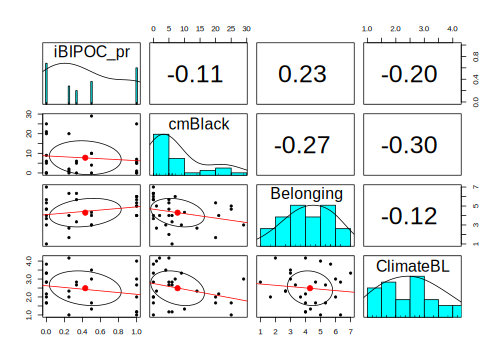
\includegraphics{ReC_MultivariateModeling_files/figure-latex/pairs panels-1.pdf}

The histograms displayed in the diagonal graph for us what we learned from the Shapiro Wilk's test of normality. We can clearly see the non-normal distribution in the iBIPOC\_pr and cmBlack variables.

\hypertarget{evaluating-multivariate-normality}{%
\section{Evaluating Multivariate Normality}\label{evaluating-multivariate-normality}}

\textbf{Multivariate outliers} have extreme scores on two or more variables, or a pattern of scores that is atypical. For example, a case may have scores between two and three standard deviations above the mean on all variables, even though no case would be extreme. A common method of multivariate outlier detection is the \textbf{Mahalanobis distance} (\(D_{M}^{2}\)). This indicates the distance in variance units between the profile of scores for that case and the vector of sample means, or \textbf{centroid}, correcting for intercorrelations.

The \emph{outlier()} function from the \emph{psych} package tells us how far each datapoint is from the multivariate centroid of the data. That is, find the squared Mahalanobis distance for each data point and compare it to the expected values of \(\chi^2\). The \emph{outlier()} protocol also produces a Q-Q (quantile-quantile) plot with the \emph{n} most extreme data points labeled.

The code below appends the Mahalanobis values to the dataframe. It is easy, then, to identify, sort, and examine the most extreme values (relative to the rest of the data in their case/row) to make decisions about their retention or adjustment.

Numeric variables are required in the for the calculation of the Mahalanobis.

\begin{Shaded}
\begin{Highlighting}[]
\NormalTok{item\_scores\_df}\SpecialCharTok{$}\NormalTok{Mahal }\OtherTok{\textless{}{-}}\NormalTok{ psych}\SpecialCharTok{::}\FunctionTok{outlier}\NormalTok{(item\_scores\_df[}\FunctionTok{c}\NormalTok{(}\StringTok{"iBIPOC\_pr"}\NormalTok{, }\StringTok{"cmBlack"}\NormalTok{, }\StringTok{"Belonging"}\NormalTok{, }\StringTok{"ClimateBL"}\NormalTok{)]) }
\end{Highlighting}
\end{Shaded}

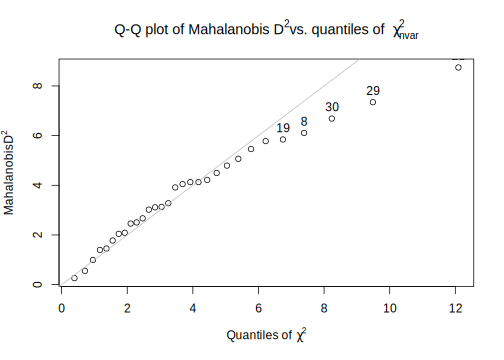
\includegraphics{ReC_MultivariateModeling_files/figure-latex/Detect multivariate outliers-1.pdf}

Q-Q plots take your sample data, sort it in ascending order, and then plot them versus quantiles (the number varies; you can see it on the X axis) calculated from a theoretical distribution. The number of quantiles is selected to match the size of your sample data. While Normal Q-Q Plots are the ones most often used in practice due to so many statistical methods assuming normality, Q-Q Plots can actually be created for any distribution. To the degree that the plotted line stays on the straight line (representing the theoretical normal distribution), the data is multivariate normally distributed.

It is possible, then to analyze the Mahalanobis distance values.

\begin{Shaded}
\begin{Highlighting}[]
\NormalTok{psych}\SpecialCharTok{::}\FunctionTok{describe}\NormalTok{(item\_scores\_df}\SpecialCharTok{$}\NormalTok{Mahal)}
\end{Highlighting}
\end{Shaded}

\begin{verbatim}
##    vars  n mean   sd median trimmed  mad  min  max range skew kurtosis   se
## X1    1 30 3.72 2.07    3.6    3.62 2.21 0.26 8.74  8.48 0.39     -0.5 0.38
\end{verbatim}

Using this information we can determine cases that have a Mahalanobis distance values that exceeds three standard deviations around the mean. In fact, we can have these noted in a column in the dataframe.

\begin{Shaded}
\begin{Highlighting}[]
\FunctionTok{library}\NormalTok{(dplyr)}
\CommentTok{\#str(item\_scores\_df$Mahal)}
\NormalTok{item\_scores\_df}\SpecialCharTok{$}\NormalTok{MOutlier }\OtherTok{\textless{}{-}} \FunctionTok{if\_else}\NormalTok{(item\_scores\_df}\SpecialCharTok{$}\NormalTok{Mahal }\SpecialCharTok{\textgreater{}}\NormalTok{ (}\FunctionTok{median}\NormalTok{(item\_scores\_df}\SpecialCharTok{$}\NormalTok{Mahal) }\SpecialCharTok{+}\NormalTok{ (}\DecValTok{3}\SpecialCharTok{*}\FunctionTok{sd}\NormalTok{(item\_scores\_df}\SpecialCharTok{$}\NormalTok{Mahal))), }\ConstantTok{TRUE}\NormalTok{, }\ConstantTok{FALSE}\NormalTok{)}

\FunctionTok{library}\NormalTok{(dplyr)}
\NormalTok{OutlierCount }\OtherTok{\textless{}{-}}\NormalTok{ item\_scores\_df}\SpecialCharTok{\%\textgreater{}\%}
  \FunctionTok{count}\NormalTok{(MOutlier)}
\NormalTok{OutlierCount}
\end{Highlighting}
\end{Shaded}

\begin{verbatim}
##   MOutlier  n
## 1    FALSE 30
\end{verbatim}

\begin{Shaded}
\begin{Highlighting}[]
\NormalTok{NumOutliers }\OtherTok{\textless{}{-}} \FunctionTok{nrow}\NormalTok{(item\_scores\_df) }\SpecialCharTok{{-}}\NormalTok{ OutlierCount}
\NormalTok{NumOutliers}
\end{Highlighting}
\end{Shaded}

\begin{verbatim}
##   MOutlier n
## 1       30 0
\end{verbatim}

\begin{Shaded}
\begin{Highlighting}[]
\FunctionTok{head}\NormalTok{(item\_scores\_df)}
\end{Highlighting}
\end{Shaded}

\begin{verbatim}
##   ID iBIPOC_pr cmBlack Belong_1 Belong_2 Belong_3 Blst_1 Blst_2 Blst_3 Blst_4
## 1  1 0.3333333       0        6        6        7      5      3      5      2
## 2  2 0.0000000       5        4        4        6      6      6      2      2
## 3  3 0.5000000      10       NA        3       NA     NA      5      2      2
## 4  4 0.3333333       6        5        3        2      2      2      2      2
## 5  5 1.0000000       5        4        4        4      6      1      1      1
## 6  6 0.0000000      20        5        6        5      5      1      1      2
##   Blst_5 Blst_6 rBlst_1 Belonging ResponseBL StigmaBL ClimateBL     Mahal
## 1      2      2       3      6.33       2.33     3.33      2.83 2.5049365
## 2      4      1       2      4.67       1.67     4.00      2.83 1.4546365
## 3     NA      2      NA        NA       2.00     3.50        NA 0.2625032
## 4      2      2       6      3.33       3.33     2.00      2.67 0.5537915
## 5      1      1       2      4.00       1.33     1.00      1.17 4.1284502
## 6      1      2       3      5.33       2.33     1.00      1.67 5.0665840
##   MOutlier
## 1    FALSE
## 2    FALSE
## 3    FALSE
## 4    FALSE
## 5    FALSE
## 6    FALSE
\end{verbatim}

CUMULATIVE CAPTURE FOR THE APA STYLE WRITE-UP: We evaluated multivariate normality with the Mahalanobis distance test. Specifically, we used the \emph{outlier()} function in the \emph{psych} package and included all continuous variables in the calculation. Our visual inspection of the Q-Q plot suggested that the plotted line strayed from the straight line as the quantiles increased. Additionally, we appended the Mahalanobis distance scores as a variable to the data. Analyzing this variable, we found that 0 exceed three standard deviations beyond the median. \emph{Thus, with no outliers, we assumed multivariate normality and proceeded with the data analysis} AS DATA IS ADDED THIS NUMBER OF OUTLIERS COULD UPDATE FROM ZERO AND THIS TEXT COULD CHANGE.

\hypertarget{a-few-words-on-transformations}{%
\section{A Few Words on Transformations}\label{a-few-words-on-transformations}}

To quote from Kline \citeyearpar{kline_principles_2016}, ``Before applying a normalizing transformation, you should think about the variables of interest and whether the expectation of normality is reasonable.'' (p.~77)

At this point in history, the non-normal distribution of the proportions of classmates who are Black and instructional staff who are BIPOC are accurate representations in higher education. Kline \citeyearpar{kline_principles_2016} has noted that transforming an inherently non-normal variable to force a normal distribution may fundamentally alter it such that the variable of interest is not actually studied. Kline's chapter reviews some options for applying corrections to outliers. Additionally, the chapter describes a variety of normalizing transformations.

On a personal note, while I will use stadardized scores (a linear transformation) if it improves interpretation and center variables around a meaningful intercept, I tend to resist the transformation of data without a really compelling reason. Why? It's complicated and can make interpretation difficult.

\hypertarget{the-apa-style-write-up-1}{%
\section{The APA Style Write-Up}\label{the-apa-style-write-up-1}}

Since the focus of this chapter was on data diagnostics, the APA style writeup will focus on on this element of the Method section:

\hypertarget{data-diagnostics}{%
\subsection{Data Diagnostics}\label{data-diagnostics}}

Data screening suggested that 31 individuals opened the survey link. Of those, 30 granted consent and proceeded to the survey items. A further inclusion criteria was that the course was taught in the U.S; 30 met this criteria.

Available item analysis (AIA; \citep{parent_handling_2013}) is a strategy for managing missing data that uses available data for analysis and excludes cases with missing data points only for analyses in which the data points would be directly involved. Parent (2013) suggested that AIA is equivalent to more complex methods (e.g., multiple imputation) across a number of variations of sample size, magnitude of associations among items, and degree of missingness. Thus, we utilized Parent's recommendations to guide our approach to managing missing data. Missing data analyses were conducted with tools in base R as well as the R packages, \emph{psych} (v. 1.0.12) and \emph{mice} (v. 3.13.0).

Across cases that were deemed eligible on the basis of the inclusion/exclusion criteria, missingness ranged from 0\% to 36\%. Across the dataset, 4.24\% of cells had missing data and 80.00\% of cases had nonmissing data. At this stage in the analysis, we allowed all cases with less than 90\% missing to continue to the scoring stage. Guided by Parent's \citeyearpar{parent_handling_2013} AIA approach, scales with three items were scored if at least two items were non-missing; the scale with four items was scored if it at least three non-missing items; and the scale with six items was scored if it had at least five non-missing items.

Across the 30 cases for which the scoring protocol was applied, missingness ranged from 0\% to 33\%. After eliminating cases with greater than 20\% missing, the dataset analyzed included 27 cases. In this dataset we had 1.23\% missing across the df; 92.59\% of the rows had nonmissing data.

Regarding the distributional characteristics of the data, skew and kurtosis values of the variables fell below the values of 3 (skew) and 8 to 20 (kurtosis) that Kline suggests are concerning \citeyearpar{kline_principles_2016}. Results of the Shapiro-Wilk test of normality indicate that our variables assessing the proportion of classmates who are Black (\(W\) = 0.815, \(p\) = 0.0001) and the proportion of BIPOC instructional staff(\(W\) = 0.811, \(p\) = 0.0002) are statistically significantly different than a normal distribution. The scales assessing the respondent's belonging (\(W\) = 0.975, \(p\) = 0.6866) and the respondent's perception of campus climate for Black students (\(W\) = 0.953, \(p\) = 0.2528) did not differ differently from a normal distribution.

We evaluated multivariate normality with the Mahalanobis distance test. Specifically, we used the \emph{outlier()} function in the \emph{psych} package and included all continuous variables in the calculation. Our visual inspection of the Q-Q plot suggested that the plotted line strayed from the straight line as the quantiles increased. Additionally, we appended the Mahalanobis distance scores as a variable to the data. Analyzing this variable, we found that 0 exceed three standard deviations beyond the median. \emph{Thus, with no outliers, we assumed multivariate normality and proceeded with the data analysis} AS DATA IS ADDED THIS NUMBER OF OUTLIERS COULD UPDATE FROM ZERO AND THIS TEXT COULD CHANGE.

Given that our sample sizes were reasonable for the planned analyses and the degree of missingness was low, we used pairwise deletion in our multiple regression analysis.

\hypertarget{a-quick-regression-of-our-research-vignette}{%
\section{A Quick Regression of our Research Vignette}\label{a-quick-regression-of-our-research-vignette}}

With some confidence that our scrubbed-and-scored variables are appropriate for analysis, let me conduct the super quick regression that is our research vignette.

\begin{figure}
\centering
\includegraphics{images/Ch04/BlStuRegression.jpg}
\caption{An image of the statistical model for which we are preparing data.}
\end{figure}

\begin{Shaded}
\begin{Highlighting}[]
\NormalTok{Climate\_fit }\OtherTok{\textless{}{-}} \FunctionTok{lm}\NormalTok{(ClimateBL }\SpecialCharTok{\textasciitilde{}}\NormalTok{ Belonging }\SpecialCharTok{+}\NormalTok{ cmBlack }\SpecialCharTok{+}\NormalTok{ iBIPOC\_pr, }\AttributeTok{data =}\NormalTok{ item\_scores\_df)}
\FunctionTok{summary}\NormalTok{(Climate\_fit)}
\end{Highlighting}
\end{Shaded}

\begin{verbatim}
## 
## Call:
## lm(formula = ClimateBL ~ Belonging + cmBlack + iBIPOC_pr, data = item_scores_df)
## 
## Residuals:
##      Min       1Q   Median       3Q      Max 
## -1.81102 -0.50885  0.06717  0.52050  1.64431 
## 
## Coefficients:
##             Estimate Std. Error t value Pr(>|t|)    
## (Intercept)  3.08986    0.64324   4.804 9.54e-05 ***
## Belonging   -0.02121    0.12995  -0.163   0.8719    
## cmBlack     -0.04980    0.02258  -2.206   0.0387 *  
## iBIPOC_pr   -0.57833    0.45679  -1.266   0.2193    
## ---
## Signif. codes:  0 '***' 0.001 '**' 0.01 '*' 0.05 '.' 0.1 ' ' 1
## 
## Residual standard error: 0.8998 on 21 degrees of freedom
##   (5 observations deleted due to missingness)
## Multiple R-squared:  0.2259, Adjusted R-squared:  0.1153 
## F-statistic: 2.043 on 3 and 21 DF,  p-value: 0.1386
\end{verbatim}

Results of a multiple regression predicting the respondents' perceptions of campus climate for Black students indicated that neither contributions of the respondents' personal belonging (\(B\) = -0.021, \(p\) = 0.872), the proportion of classmates who were Black (\(B\) = -0.050, \(p\) = 0.039), nor the proportion of BIPOC instructional staff (\(B\) = -0.578, \(p\) = 0.219) led to statistically significant changes in perceptions of campus climate for Black students. Results are presented in Table 2.

\begin{Shaded}
\begin{Highlighting}[]
\FunctionTok{library}\NormalTok{(apaTables)}
\FunctionTok{apa.cor.table}\NormalTok{(item\_scores\_df[}\FunctionTok{c}\NormalTok{(}\StringTok{"iBIPOC\_pr"}\NormalTok{, }\StringTok{"cmBlack"}\NormalTok{, }\StringTok{"Belonging"}\NormalTok{, }\StringTok{"ClimateBL"}\NormalTok{)], }\AttributeTok{table.number =} \DecValTok{1}\NormalTok{, }\AttributeTok{show.sig.stars =} \ConstantTok{TRUE}\NormalTok{, }\AttributeTok{filename =} \StringTok{"Table1\_M\_SDs\_r\_DataDx"}\NormalTok{)}
\end{Highlighting}
\end{Shaded}

\begin{verbatim}
## 
## 
## Table 1 
## 
## Means, standard deviations, and correlations with confidence intervals
##  
## 
##   Variable     M    SD   1           2            3          
##   1. iBIPOC_pr 0.43 0.41                                     
##                                                              
##   2. cmBlack   7.07 7.82 -.14                                
##                          [-.49, .25]                         
##                                                              
##   3. Belonging 4.35 1.51 .24         -.23                    
##                          [-.15, .57] [-.55, .15]             
##                                                              
##   4. ClimateBL 2.47 0.98 -.21        -.39*        -.10       
##                          [-.56, .20] [-.67, -.01] [-.46, .29]
##                                                              
## 
## Note. M and SD are used to represent mean and standard deviation, respectively.
## Values in square brackets indicate the 95% confidence interval.
## The confidence interval is a plausible range of population correlations 
## that could have caused the sample correlation (Cumming, 2014).
##  * indicates p < .05. ** indicates p < .01.
## 
\end{verbatim}

\begin{Shaded}
\begin{Highlighting}[]
\FunctionTok{library}\NormalTok{(apaTables)}
\NormalTok{apaTables}\SpecialCharTok{::}\FunctionTok{apa.reg.table}\NormalTok{(Climate\_fit, }\AttributeTok{table.number =} \DecValTok{2}\NormalTok{, }\AttributeTok{filename =} \StringTok{"Climate\_table.doc"}\NormalTok{)}
\end{Highlighting}
\end{Shaded}

\begin{verbatim}
## 
## 
## Table 2 
## 
## Regression results using ClimateBL as the criterion
##  
## 
##    Predictor      b       b_95%_CI  beta    beta_95%_CI sr2  sr2_95%_CI     r
##  (Intercept) 3.09**   [1.75, 4.43]                                           
##    Belonging  -0.02  [-0.29, 0.25] -0.03  [-0.45, 0.38] .00 [-.02, .02]  -.00
##      cmBlack -0.05* [-0.10, -0.00] -0.43 [-0.84, -0.02] .18 [-.09, .45] -.40*
##    iBIPOC_pr  -0.58  [-1.53, 0.37] -0.25  [-0.66, 0.16] .06 [-.10, .22]  -.21
##                                                                              
##                                                                              
##                                                                              
##              Fit
##                 
##                 
##                 
##                 
##        R2 = .226
##  95% CI[.00,.42]
##                 
## 
## Note. A significant b-weight indicates the beta-weight and semi-partial correlation are also significant.
## b represents unstandardized regression weights. beta indicates the standardized regression weights. 
## sr2 represents the semi-partial correlation squared. r represents the zero-order correlation.
## Square brackets are used to enclose the lower and upper limits of a confidence interval.
## * indicates p < .05. ** indicates p < .01.
## 
\end{verbatim}

\hypertarget{practice-problems-2}{%
\section{Practice Problems}\label{practice-problems-2}}

The three problems described below are designed to be continuations from the previous chapter (Scrubbing).

\hypertarget{problem-1-reworking-the-chapter-problem-1}{%
\subsection{Problem \#1: Reworking the Chapter Problem}\label{problem-1-reworking-the-chapter-problem-1}}

If you chose this option in the prior chapters, you imported the data from Qualtrics, applied inclusion/exclusion criteria, renamed variables, downsized the df to the variables of interest, properly formatted the variables, interpreted item-level missingness, scored the scales/subscales, interpreted scale-level missingness, and wrote up the results.

If you continue with this option, please continue working with the data to:

Continue working with this data to:

\begin{longtable}[]{@{}
  >{\raggedright\arraybackslash}p{(\columnwidth - 4\tabcolsep) * \real{0.76}}
  >{\centering\arraybackslash}p{(\columnwidth - 4\tabcolsep) * \real{0.12}}
  >{\centering\arraybackslash}p{(\columnwidth - 4\tabcolsep) * \real{0.11}}@{}}
\toprule
Assignment Component & & \\
\midrule
\endhead
1. Calculate alpha coefficients for scales/subscales. & 5 & \_\_\_\_\_ \\
2. Evaluate univariate normality (skew, kurtosis, Shapiro-Wilks). & 5 & \_\_\_\_\_ \\
3. Evaluate multivarite normality (Mahalanobis test) & 5 & \_\_\_\_\_ \\
4. Represent your work in an APA-style write-up (added to the writeup in the previous chapter) & 5 & \_\_\_\_\_ \\
5. For fun, run a quick analysis (e.g., regression, ANOVA) including at least three variables & 5 & \_\_\_\_\_ \\
6. Explanation to grader & 5 & \_\_\_\_\_ \\
\textbf{Totals} & 30 & \_\_\_\_\_ \\
\bottomrule
\end{longtable}

\hypertarget{problem-2-use-the-rate-a-recent-course-survey-choosing-different-variables-2}{%
\subsection{\texorpdfstring{Problem \#2: Use the \emph{Rate-a-Recent-Course} Survey, Choosing Different Variables}{Problem \#2: Use the Rate-a-Recent-Course Survey, Choosing Different Variables}}\label{problem-2-use-the-rate-a-recent-course-survey-choosing-different-variables-2}}

If you chose this option in the prior chapter, you chose a minimum of three variables from the \emph{Rate-a-Recent-Course} survey to include in a simple statistical model. You imported the data from Qualtrics, applied inclusion/exclusion criteria, renamed variables, downsized the df to the variables of interest, properly formatted the variables, interpreted item-level missingness, scored the scales/subscales, interpreted scale-level missingness, and wrote up the results.

Continue working with this data to:

\begin{longtable}[]{@{}
  >{\raggedright\arraybackslash}p{(\columnwidth - 4\tabcolsep) * \real{0.76}}
  >{\centering\arraybackslash}p{(\columnwidth - 4\tabcolsep) * \real{0.12}}
  >{\centering\arraybackslash}p{(\columnwidth - 4\tabcolsep) * \real{0.11}}@{}}
\toprule
Assignment Component & & \\
\midrule
\endhead
1. Calculate alpha coefficients for scales/subscales. & 5 & \_\_\_\_\_ \\
2. Evaluate univariate normality (skew, kurtosis, Shapiro-Wilks). & 5 & \_\_\_\_\_ \\
3. Evaluate multivarite normality (Mahalanobis test) & 5 & \_\_\_\_\_ \\
4. Represent your work in an APA-style write-up (added to the writeup in the previous chapter) & 5 & \_\_\_\_\_ \\
5. For fun, run a quick analysis (e.g., regression, ANOVA) including at least three variables & 5 & \_\_\_\_\_ \\
6. Explanation to grader & 5 & \_\_\_\_\_ \\
\textbf{Totals} & 30 & \_\_\_\_\_ \\
\bottomrule
\end{longtable}

\hypertarget{problem-3-other-data-2}{%
\subsection{Problem \#3: Other data}\label{problem-3-other-data-2}}

If you chose this option in the prior chapter, you used raw data that was available to you. You imported it into R, applied inclusion/exclusion criteria, renamed variables, downsized the df to the variables of interest, properly formatted the variables, interpreted item-level missingness, scored the scales/subscales, interpreted scale-level missingness, and wrote up the results.

Continue working with this data to:

\begin{longtable}[]{@{}
  >{\raggedright\arraybackslash}p{(\columnwidth - 4\tabcolsep) * \real{0.76}}
  >{\centering\arraybackslash}p{(\columnwidth - 4\tabcolsep) * \real{0.12}}
  >{\centering\arraybackslash}p{(\columnwidth - 4\tabcolsep) * \real{0.11}}@{}}
\toprule
Assignment Component & & \\
\midrule
\endhead
1. Calculate alpha coefficients for scales/subscales. & 5 & \_\_\_\_\_ \\
2. Evaluate univariate normality (skew, kurtosis, Shapiro-Wilks). & 5 & \_\_\_\_\_ \\
3. Evaluate multivarite normality (Mahalanobis test) & 5 & \_\_\_\_\_ \\
4. Represent your work in an APA-style write-up (added to the writeup in the previous chapter) & 5 & \_\_\_\_\_ \\
5. For fun, run a quick analysis (e.g., regression, ANOVA) including at least three variables & 5 & \_\_\_\_\_ \\
6. Explanation to grader & 5 & \_\_\_\_\_ \\
\textbf{Totals} & 30 & \_\_\_\_\_ \\
\bottomrule
\end{longtable}

\hypertarget{references-2}{%
\section{References}\label{references-2}}

\begin{Shaded}
\begin{Highlighting}[]
\FunctionTok{sessionInfo}\NormalTok{()}
\end{Highlighting}
\end{Shaded}

\begin{verbatim}
## R version 4.0.4 (2021-02-15)
## Platform: x86_64-w64-mingw32/x64 (64-bit)
## Running under: Windows 10 x64 (build 18362)
## 
## Matrix products: default
## 
## locale:
## [1] LC_COLLATE=English_United States.1252 
## [2] LC_CTYPE=English_United States.1252   
## [3] LC_MONETARY=English_United States.1252
## [4] LC_NUMERIC=C                          
## [5] LC_TIME=English_United States.1252    
## 
## attached base packages:
## [1] stats     graphics  grDevices utils     datasets  methods   base     
## 
## other attached packages:
##  [1] apaTables_2.0.8   psych_2.0.12      mice_3.13.0       sjstats_0.18.0   
##  [5] formattable_0.2.1 forcats_0.5.0     stringr_1.4.0     dplyr_1.0.2      
##  [9] purrr_0.3.4       readr_1.4.0       tidyr_1.1.2       tibble_3.0.4     
## [13] ggplot2_3.3.3     tidyverse_1.3.0   qualtRics_3.1.4  
## 
## loaded via a namespace (and not attached):
##  [1] nlme_3.1-151      fs_1.5.0          lubridate_1.7.9.2 MBESS_4.8.0      
##  [5] insight_0.11.1    httr_1.4.2        tools_4.0.4       backports_1.2.0  
##  [9] R6_2.5.0          sjlabelled_1.1.7  DBI_1.1.0         colorspace_2.0-0 
## [13] withr_2.3.0       tidyselect_1.1.0  mnormt_2.0.2      emmeans_1.5.3    
## [17] curl_4.3          compiler_4.0.4    performance_0.6.1 cli_2.2.0        
## [21] rvest_0.3.6       xml2_1.3.2        sandwich_3.0-0    bookdown_0.21    
## [25] bayestestR_0.8.0  scales_1.1.1      mvtnorm_1.1-1     digest_0.6.27    
## [29] minqa_1.2.4       rmarkdown_2.6     pkgconfig_2.0.3   htmltools_0.5.0  
## [33] lme4_1.1-26       dbplyr_2.0.0      htmlwidgets_1.5.3 rlang_0.4.9      
## [37] readxl_1.3.1      rstudioapi_0.13   generics_0.1.0    zoo_1.8-8        
## [41] jsonlite_1.7.2    magrittr_2.0.1    parameters_0.10.1 Matrix_1.2-18    
## [45] Rcpp_1.0.5        munsell_0.5.0     fansi_0.4.1       lifecycle_0.2.0  
## [49] stringi_1.5.3     multcomp_1.4-15   yaml_2.2.1        MASS_7.3-53      
## [53] grid_4.0.4        parallel_4.0.4    sjmisc_2.8.5      crayon_1.3.4     
## [57] lattice_0.20-41   haven_2.3.1       splines_4.0.4     hms_0.5.3        
## [61] tmvnsim_1.0-2     knitr_1.30        pillar_1.4.7      boot_1.3-25      
## [65] estimability_1.3  effectsize_0.4.1  codetools_0.2-18  reprex_0.3.0     
## [69] glue_1.4.2        evaluate_0.14     modelr_0.1.8      vctrs_0.3.6      
## [73] nloptr_1.2.2.2    cellranger_1.1.0  gtable_0.3.0      assertthat_0.2.1 
## [77] xfun_0.19         xtable_1.8-4      broom_0.7.3       coda_0.19-4      
## [81] survival_3.2-7    statmod_1.4.35    TH.data_1.0-10    ellipsis_0.3.1
\end{verbatim}

  \bibliography{STATSnMETH.bib}

\end{document}
